\chapter{Partitioned finite element method}\label{ch:pfem}

\epigraph{Every truth is simple\dots is that not doubly a lie?}{\textit{Twilight of the Idols \\ Friedrich Nietzsche}}

\minitoc

\lettrine{\color{theme}{D}}iscretization is the process of transferring continuous models into discrete counterparts. The discrete model should be faithful to the continuous one. To this aim, it is usually essential that the main properties of the continuous system are preserved at the discrete level. An algorithm that is capable of conserving properties at the discrete level is called structure-preserving \cite{christiansen2011}. In this chapter, a method to spatially discretize infinite-dimensional pHs into finite-dimensional ones in a structure preserving manner is illustrated.

\section{Discretization under uniform boundary condition}
A discrete version of a infinite-dimensional pH system is meant to preserve the underlying properties related to power continuity. To achieve this purpose, the discretization procedure consists of two steps \cite{kotyczka2018weak}:
\begin{itemize}
	\item Finite-dimensional approximation of the Stokes-Dirac structure, i.e. the formally skew symmetric differential operator that defines the structure. The duality of the power variables has to be mapped onto the finite approximation. The subspace of the discrete variables will be represented by a Dirac structure. 
	\item The Hamiltonian requires as well a suitable discretization, which gives rise to a discrete Hamiltonian. 
\end{itemize} 
A structure-preserving discretization is able to construct an equivalent pH system that possesses the structural properties of the original model:
\begin{tcbraster}[raster columns=2, raster equal height]
	\begin{tcolorbox}[width=0.4\textwidth, nobeforeafter, colframe=theme,title=Infinite dimensional pH system]%%
		PDE with distributed inputs:
		\begin{align*}
		\diffp{\bm{\alpha}}{t}(\bm{x}, t) &= \mathcal{J} {\displaystyle \diffd{H}{\bm{\alpha}}}+ \mathcal{B} \textcolor{red}{\bm{u}_\Omega(\bm{x}, t)}, \\
		\textcolor{red}{\bm{y}_\Omega(\bm{x}, t)} &= \mathcal{B}^* {\displaystyle \diffd{H}{\bm{\alpha}}}.
		\end{align*}
		Boundary conditions: 
		\[\textcolor{blue}{\bm{u}_\partial} = \mathcal{B}_\partial{\displaystyle \diffd{H}{\bm{\alpha}}}, \quad \textcolor{blue}{\bm{y}_\partial} = \mathcal{C}_\partial {\displaystyle \diffd{H}{\bm{\alpha}}}. \]
		Power balance (Stokes Theorem): 
		\[ \dot{H} = \displaystyle \int_{\partial \Omega} \textcolor{blue}{\bm{u}_\partial} \cdot \textcolor{blue}{\bm{y}_\partial} \d{S} +  \int_{\Omega} \textcolor{red}{\bm{u}_\Omega} \cdot \textcolor{red}{\bm{y}_\Omega} \d{\Omega}.
		\]
	\end{tcolorbox} 
	\begin{tcolorbox}[width=0.4\textwidth, nobeforeafter,  colframe=theme,title=Structure-preserving discretization]%%
		Resulting ODE:
		\begin{align*}
		\dot{\bm{\alpha}}_d &= \mathbf{J} \, {\nabla {H}_d} + \mathbf{B}_\Omega \textcolor{red}{\mathbf{u}_\Omega} + \mathbf{B}_\partial \textcolor{blue}{\mathbf{u}_\partial}, \\
		\textcolor{red}{\mathbf{y}_\Omega} &= \mathbf{B}_\Omega^\top \, {\nabla {H}_d}, \\
		\textcolor{blue}{\mathbf{y}_\partial} &= \mathbf{B}_\partial^\top \,{\nabla {H}_d}.
		\end{align*}
		Discretized Hamiltonian:
		\[
		H_d := H(\bm{\alpha} \equiv \bm{\alpha}_d).
		\]
		Power balance: 
		\[ \dot{H} = \textcolor{blue}{\mathbf{u}_\partial^\top \mathbf{y}_\partial} +  \textcolor{red}{\mathbf{u}_\Omega^\top \mathbf{y}_\Omega}.
		\]
	\end{tcolorbox}
\end{tcbraster}
\vspace{.5cm}
In this thesis the Partitioned Finite Element Method (PFEM), originally presented in \cite{cardoso2018pfem,cardoso2019partitioned}, is chosen to obtain discretized models of dpHs. This procedure boils down to three simple steps
\begin{enumerate}
	\item The system is written in weak form; 
	\item An integration by parts is applied to highlight the appropriate boundary control;
	\item A Galerkin method is employed to obtain a finite-dimensional system. For the approximation basis the finite element method is here employed but spectral methods can be used as well.
\end{enumerate}

Once the system has been put into weak form, a subset of the equations is integrated by parts, so that boundary variables are naturally included into the formulation and appear as control inputs, the collocated outputs being defined accordingly. The discretization of energy and co-energy variables (and the associated test functions) leads directly to a full rank representation for the finite-dimensional pH system.  This approach makes possible the usage of FEM software, like FEniCS \cite{logg2012}, or Firedrake \cite{rathgeber2017firedrake}. The procedure is universal, as it relies on a general integration by parts formula that characterizes multi-dimensional pHs. This is why the methodology is illustrated in all its generality and then detailed for some particular examples.  \\

This methodology is easily applicable under a uniform causality assumption. The case of mixed boundary conditions requires additional care and will be treated in the subsequent Section \secref{sec:mixedbc}.


\subsection{General procedure}\label{sec:pfem_gen}
Given an open connected set $\Omega \in \mathbb{R}^d,\, d \in  \{1,2,3\}$, consider a generic pH system defined on~$\Omega$
\begin{subequations}
\label{eq:pHsys_2}
\begin{align}
\partial_t {\bm{\alpha}} &= \mathcal{J}\displaystyle \bm{e}, \qquad \;\;\, \bm{\alpha} \in L^2(\Omega, \mathbb{F}), \quad \mathcal{J}: L^2(\Omega, \mathbb{F}) \rightarrow L^2(\Omega, \mathbb{F}) \vert \;  \mathcal{J} = - \mathcal{J}^*, \label{eq:pHsys_dyn} \vspace{3pt}\\
\bm{e} :&= \displaystyle \delta_{\bm{\alpha}}H, \qquad \;\, \bm{e} \in H^\mathcal{J} :=\left\{\bm{e} \in L^2(\Omega, \mathbb{F}) \vert \; \mathcal{J}\bm{e} \in L^2(\Omega, \mathbb{F})  \right\}, \label{eq:pHsys_const} \\
\bm{u}_\partial &= \mathcal{B}_\partial  \displaystyle \bm{e}, \qquad \bm{u}_\partial \in \mathbb{R}^m, \label{eq:pHsys_u} \vspace{3pt}\\
\bm{y}_\partial &= \mathcal{C}_\partial \displaystyle \bm{e}, \qquad \; \bm{y}_\partial \in \mathbb{R}^m. \label{eq:pHsys_y} \vspace{3pt}
\end{align}
\end{subequations}
The operator $\mathcal{J}: L^2(\Omega, \mathbb{F}) \rightarrow L^2(\Omega, \mathbb{F})$ is a differential, formally skew adjoint operator $\mathcal{J} = - \mathcal{J}^*$ over the space $L^2(\Omega, \mathbb{F})$. The  set $\mathbb{F}$ is an appropriate Cartesian product of either scalar, vectorial or tensorial quantities. Its precise definition depends on the example upon consideration. For scalars $(a,b) \in L^2(\Omega)$, vectors $(\bm{a}, \bm{b})\in L^2(\Omega, \mathbb{R}^d)$ and tensors  $(\bm{A}, \bm{B}) \in L^2(\Omega,\mathbb{R}^{d\times d})$ the $L^2$ inner product is given by 
\begin{equation}
\inner[L^2(\Omega)]{a}{b} = \int_{\Omega} a b \d\Omega, \qquad \inner[L^2(\Omega, \mathbb{R}^d)]{\bm{a}}{\bm{b}} = \int_{\Omega} \bm{a} \cdot \bm{b} \d\Omega, \qquad \inner[L^2(\Omega, \mathbb{R}^{d \times d})]{\bm{A}}{\bm{B}} = \int_{\Omega} \bm{A} \cddot \bm{B} \d\Omega.
\end{equation} 
For scalars ${a}_\partial, {b}_\partial \in L^2(\partial\Omega)$ and vectors  $\bm{a}_\partial, \bm{b}_\partial \in L^2(\partial\Omega, \mathbb{R}^m)$ defined on the boundary the inner product is defined as
\begin{equation}
\inner[L^2(\partial\Omega)]{a_\partial}{b_\partial} = \int_{\partial\Omega} a_\partial b_\partial \d{S}, \qquad \inner[L^2(\partial\Omega, \mathbb{R}^m)]{\bm{a}_\partial}{\bm{b}_\partial} = \int_{\partial\Omega} \bm{a}_\partial \cdot \bm{b}_\partial \d{S}.
\end{equation} 
 The Hamiltonian functional of Eq. \eqref{eq:pHsys_const} is allowed to be non linear in the energy variables
\begin{equation*}
H = \int_\Omega \mathcal{H}(\bm{\alpha}) \d\Omega,
\end{equation*}
where $\mathcal{H}(\bm{\alpha}): L^2(\Omega, \mathbb{F}) \rightarrow \mathbb{R}$ is a non linear function.
\\

To applied this methodology the non linearities are restricted to the Hamiltonian and a uniform causality condition is supposed to characterize the system. It is required as well that the system admits a partition of the variables. This requirement is always encountered in the following examples. These hypotheses are resumed in the following assumptions.

\begin{assumption}[Partitioning of the system]
	\label{ass:linJ}
	Consider system \eqref{eq:pHsys_dyn}. It is assumed that the Hilbert space $L^2(\Omega, \mathbb{F}) := L^2(\Omega, \mathbb{F})$ admits the splitting $L^2(\Omega, \mathbb{F}) = L^2(\Omega, \mathbb{A}) \times L^2(\Omega, \mathbb{B})$  This means that $\mathbb{F} = \mathbb{A} \times \mathbb{B}$. \\
	
	The operator $\mathcal{J}$ is assumed to be skew-symmetric (or formally skew-adjoint) on $L^2(\Omega, \mathbb{F})$ and linear:
	\begin{equation}\label{eq:assJ}
	\mathcal{J} = \mathcal{J}_{{a}} + \mathcal{J}_{{d}},
	\end{equation}
	where $\mathcal{J}_{\text{a}}$ is the algebraic contribution (a skew-symmetric matrix) and $\mathcal{J}_{\text{d}}$ the differential contribution. The algebraic part is assumed to take the form
	\begin{equation}\label{eq:assJa}
		\mathcal{J}_{{a}} = \begin{bmatrix}
		0 & -\bm{L}^\top \\
		\bm{L} & 0 \\
		\end{bmatrix}, \qquad 
		\begin{aligned}
		&\bm{L}^\top : L^2(\Omega, \mathbb{B}) \rightarrow L^2(\Omega, \mathbb{A}), \\
		&\bm{L}\;\, : L^2(\Omega, \mathbb{A}) \rightarrow L^2(\Omega, \mathbb{B}), \\
		\end{aligned}
	\end{equation}
	where $\bm{L}$ is a bounded operator. 	Analogously, the linear differential operator $\mathcal{J}_{{d}}$ is assumed to be of the form
	\begin{equation}\label{eq:assJd}
	\mathcal{J}_{\text{d}} = 
	\begin{bmatrix}
	0 & -\mathcal{L}^* \\
	\mathcal{L} & 0 \\
	\end{bmatrix}, \qquad 
	\begin{aligned}
	&\mathcal{L}^* : L^2(\Omega, \mathbb{B}) \rightarrow L^2(\Omega, \mathbb{A}), \\
	&\mathcal{L}\;\, : L^2(\Omega, \mathbb{A}) \rightarrow L^2(\Omega, \mathbb{B}), \\
	\end{aligned}
	\end{equation}
	where $\mathcal{L}^*$ denotes the formal adjoint of the linear differential operator $\mathcal{L}$. 	The operator $\mathcal{L}$ is unbounded and  can be either a first or a second order differential operator (in the latter case it can be expressed as $\mathcal{L} = \mathcal{L}_1 \circ \mathcal{L}_2$). Given the splitting $L^2(\Omega, \mathbb{A}) \times L^2(\Omega, \mathbb{B}) = L^2(\Omega, \mathbb{F})$ the Hilbert space $H^\mathcal{J}$ can be split as well as 
	\begin{equation}
		H^\mathcal{J} = H^\mathcal{L} \times H^\mathcal{-L^*}, \qquad
		\begin{aligned}
		H^\mathcal{L} &:= \left\{\bm{u}_1 \in L^2(\Omega, \mathbb{A}) \vert \; \mathcal{L}\bm{u}_1 \in L^2(\Omega, \mathbb{B}) \right\}, \\
		H^\mathcal{-L^*} &:= \left\{\bm{u}_2 \in L^2(\Omega, \mathbb{B}) \vert \; -\mathcal{L}^*\bm{u}_2 \in L^2(\Omega, \mathbb{A}) \right\}
		\end{aligned}
	\end{equation}
\end{assumption}

\begin{remark}
	Notice that this assumption is also made in \cite{skrepek2019wellposedness} (using a vectorial notation for tensors) to demonstrate the well-posedness of linear pHs in arbitrary geometrical domains.
\end{remark}

The boundary operators are then supposed to fulfill the following assumption, that guarantees a uniform causality condition.

\begin{assumption}[Abstract integration by parts formula]
	\label{ass:operBC}
	Assume that there exist  two boundary operators $\mathcal{N}_{\partial, 1}, \; \mathcal{N}_{\partial, 2}$ such that for $(\bm{u}_1, \bm{u}_2) \in H^\mathcal{L} \times H^\mathcal{-L^*}$ a general integration by parts formula holds
	\begin{equation}\label{eq:intbypartsL} 
	\inner[L^2(\Omega, \mathbb{B})]{\bm{u}_2}{\mathcal{L}\,\bm{u}_1} - \inner[L^2(\Omega, \mathbb{A})]{\mathcal{L}^* \, \bm{u}_2}{\bm{u}_1} = \inner[L^2(\partial \Omega, \mathbb{R}^m)]{\mathcal{N}_{\partial, 1} \bm{u}_1}{\mathcal{N}_{\partial, 2} \bm{u}_2}. 
	\end{equation}
	The boundary operators $\mathcal{B}_\partial, \, \mathcal{C}_\partial$ of Eqs. \eqref{eq:pHsys_u}, \eqref{eq:pHsys_y}, are then assumed to verify, in an exclusive manner, either
	\begin{equation}\label{eq:assB2C1}
	\mathcal{B}_\partial = \begin{bmatrix}
	0 & \mathcal{N}_{\partial, 2} \\
	\end{bmatrix}, \quad 
	\mathcal{C}_\partial = \begin{bmatrix}
	\mathcal{N}_{\partial, 1} & 0 \\
	\end{bmatrix},
	\end{equation}
	or 
	\begin{equation}\label{eq:assB1C2}
	\mathcal{B}_\partial = \begin{bmatrix}
	\mathcal{N}_{\partial, 1} & 0 \\
	\end{bmatrix}, \quad \mathcal{C}_\partial = \begin{bmatrix}
	0 & \mathcal{N}_{\partial, 2} \\
	\end{bmatrix}.
	\end{equation}

\end{assumption}

\begin{remark}[Duality pairing for rigged Hilbert spaces]
	The integration by part formula establishes a duality pairing between Sobolev spaces. This duality pairing is then compatible with an $L^2$ inner product in presence of a rigged Hilbert space (or Gelfand triple \cite{gel1964generalized}). Without entering into technical details, we shall always use this equivalence of representation. Therefore, the boundary integrals are  expressed as $L^2$ inner product over the boundary. 
\end{remark}

Thanks to Assumption \ref{ass:linJ}, System \eqref{eq:pHsys_2} is rewritten as 
\begin{subequations}
	\label{eq:pHsys_ass} 
	\begin{align}
	\partial_t \begin{pmatrix}
	{\bm{\alpha}}_1 \\ {\bm{\alpha}}_2
	\end{pmatrix} &= \begin{bmatrix}
	0 & -\bm{L}^\top - \mathcal{L}^* \\
	\bm{L} + \mathcal{L} & 0 \\
	\end{bmatrix}\begin{pmatrix}
	\bm{e}_1 \\ \bm{e}_2
	\end{pmatrix} , \qquad \begin{aligned}
	\bm{\alpha}_1 \in L^2(\Omega, \mathbb{A}), 	\\
	\bm{\alpha}_2 \in L^2(\Omega, \mathbb{B}), 
	\end{aligned} \label{eq:pHsys_dyn_ass} \vspace{3pt}\\
	\begin{pmatrix}
	\bm{e}_1 \\ \bm{e}_2
	\end{pmatrix} &:= \begin{pmatrix}
	\delta_{\bm{\alpha}_1}H \\ \delta_{\bm{\alpha}_2}H
	\end{pmatrix} , \qquad \begin{aligned}
	\bm{e}_1 &\in H^\mathcal{L}, 	\\
	\bm{e}_2 &\in H^{-\mathcal{L}^*}.
	\end{aligned} \label{eq:pHsys_const_ass} 
	\end{align}
\end{subequations}
In light of Assumption \ref{ass:operBC}, if Eq. \eqref{eq:assB2C1} holds the boundary variables are given by 
\begin{equation}\label{eq:pHsys_assB2C1}
\bm{u}_\partial = \mathcal{N}_2 \displaystyle \bm{e}_2, \qquad  \bm{y}_\partial = \mathcal{N}_1 \displaystyle \bm{e}_1, \qquad  \bm{u}_\partial,\, \bm{y}_\partial \in \mathbb{R}^m.
\end{equation}
Otherwise, if Eq. \eqref{eq:assB1C2} applies, then
\begin{equation}\label{eq:pHsys_assB1C2}
\bm{u}_\partial = \mathcal{N}_1 \displaystyle \bm{e}_1, \qquad 
\bm{y}_\partial = \mathcal{N}_2 \displaystyle \bm{e}_2, \qquad  \bm{u}_\partial,\, \bm{y}_\partial \in \mathbb{R}^m. 
\end{equation}
In both cases, the power balance reads
\begin{equation}\label{eq:powbal_2}
\begin{aligned}
\dot{H} &= \inner[L^2(\Omega, \mathbb{A})]{\bm{e}_1}{\partial_{t} \bm{\alpha}_1} + \inner[L^2(\Omega, \mathbb{B})]{\bm{e}_2}{\partial_{t} \bm{\alpha}_2}, \\
&=\inner[L^2(\Omega, \mathbb{A})]{\bm{e}_1}{-\mathcal{L}^* \bm{e}_2} + \inner[L^2(\Omega, \mathbb{B})]{\bm{e}_2}{\mathcal{L} \bm{e}_1}, \\
&= \inner[L^2(\partial \Omega, \mathbb{R}^m)]{\mathcal{N}_{\partial, 1} \bm{e}_1}{\mathcal{N}_{\partial, 2} \bm{e}_2}, \\
&= \inner[L^2(\partial \Omega, \mathbb{R}^m)]{\bm{y}_\partial}{\bm{u}_\partial}.
\end{aligned}
\end{equation}
We are now in a position to illustrate the methodology. 
\paragraph{Step 1} First consider the weak form of system \eqref{eq:pHsys_dyn_ass}, obtained by taking the $L^2$ inner product introducing an appropriate test function $\bm{v} = (\bm{v}_1, \bm{v}_2) \in \mathbb{A} \times \mathbb{B} = \mathbb{F}$ and integrating over the domain $\Omega$
\begin{equation}\label{eq:weak_dyn}
\begin{aligned}
\inner[L^2(\Omega, \mathbb{A})]{\bm{v}_1}{\partial_t \bm{\alpha}_1} &= -  \langle{\bm{v}_1},\,{\bm{L}^\top \bm{e}_2}\rangle_{L^2(\Omega, \mathbb{A})} -  \inner[L^2(\Omega, \mathbb{A})]{\bm{v}_1}{\mathcal{L}^*\bm{e}_2}, \\
\inner[L^2(\Omega, \mathbb{B})]{\bm{v}_2}{\partial_t \bm{\alpha}_2} &= \inner[L^2(\Omega, \mathbb{B})]{\bm{v}_2}{\bm{L}\bm{e}_1}+ \inner[L^2(\Omega, \mathbb{B})]{\bm{v}_2}{\mathcal{L}\bm{e}_1}.
\end{aligned}
\end{equation}



To obtain a closed system, the constitutive law \eqref{eq:pHsys_const_ass} and the output variables \eqref{eq:pHsys_y} are put in weak form
\begin{equation}
\begin{aligned}
\inner[L^2(\Omega, \mathbb{A})]{\bm{v}_1}{\bm{e}_1}&= \inner[L^2(\Omega, \mathbb{A})]{\bm{v}_1}{\delta_{\bm{\alpha}_1} H}, \\
\inner[L^2(\Omega, \mathbb{B})]{\bm{v}_2}{\bm{e}_2}&= \inner[L^2(\Omega, \mathbb{B})]{\bm{v}_2}{\delta_{\bm{\alpha}_2} H}, \\
\inner[L^2(\partial \Omega, \mathbb{R}^m)]{\bm{v}_\partial}{\bm{y}_\partial} &= \inner[L^2(\partial \Omega, \mathbb{R}^m)]{\bm{v}_\partial}{\mathcal{C}_\partial \bm{e}},
\end{aligned}
\end{equation}
where the test function $\bm{v}_\partial \in L^2(\partial \Omega, \mathbb{R}^m)$ is defined on the boundary $\partial\Omega$ and $\mathcal{C}_\partial$ is defined either by Eq. \eqref{eq:assB2C1} or  \eqref{eq:assB1C2}.


\paragraph{Step 2} Next the integration by part has to be carried out. The choice is dictated by the boundary control to be imposed on the system. Consider again Eq. \eqref{eq:weak_dyn}. The integration by parts can be carried out either on term $-\inner[L^2(\Omega, \mathbb{A})]{\bm{v}_1}{\mathcal{L}^*\bm{e}_2}$, or on term $\inner[L^2(\Omega, \mathbb{B})]{\bm{v}_2}{\mathcal{L}\bm{e}_1}$. Depending on which line undergoes the integration by parts (this is why the name Partitioned Finite Element method), two structure preserving weak forms are obtained. These differ by the boundary causality imposed to the system. 


\subparagraph{Integration by parts of the term $-\inner[L^2(\Omega, \mathbb{A})]{\bm{v}_1}{\mathcal{L}^*\bm{e}_2}$}
In this case case, using Eq. \eqref{eq:intbypartsL}, it is obtained 
\begin{equation}
-\inner[L^2(\Omega, \mathbb{A})]{\bm{v}_1}{\mathcal{L}^*\bm{e}_2} = -\inner[L^2(\Omega, \mathbb{B})]{\mathcal{L}\bm{v}_1}{\bm{e}_2} + \inner[L^2(\partial \Omega, \mathbb{R}^m)]{\mathcal{N}_{\partial, 1} \bm{v}_1}{\mathcal{N}_{\partial, 2} \bm{e}_2}.
\end{equation}
Then the weak form of the system dynamics  reads 
\begin{equation}\label{eq:weak_dyn_intJ1}
\begin{aligned}
\inner[L^2(\Omega, \mathbb{A})]{\bm{v}_1}{\partial_t \bm{\alpha}_1} &=   -  \langle{\bm{v}_1}, \,{\bm{L}^\top \bm{e}_2}\rangle_{L^2(\Omega, \mathbb{A})}  -\inner[L^2(\Omega, \mathbb{B})]{\mathcal{L}\bm{v}_1}{\bm{e}_2} + \inner[L^2(\partial \Omega, \mathbb{R}^m)]{\mathcal{N}_{\partial, 1} \bm{v}_1}{\bm{u}_\partial}, \\
\inner[L^2(\Omega, \mathbb{B})]{\bm{v}_2}{\partial_t \bm{\alpha}_2} &=   \inner[L^2(\Omega, \mathbb{B})]{\bm{v}_2}{\bm{L}\bm{e}_1} + \inner[L^2(\Omega, \mathbb{B})]{\bm{v}_2}{\mathcal{L}\bm{e}_1},
\end{aligned}
\end{equation}
The following proposition is crucial as the lossless character of the infinite-dimensional system (due to the formally skew-adjoint operator) translates into an equivalent property for the corresponding bilinear form in the weak form.
\begin{proposition}
	Given the Hilbert space $H^{\mathcal{L}}_2 := H^\mathcal{L} \times L^2(\Omega, \mathbb{B})$ and variables $\bm{v} = (\bm{v}_1, \bm{v}_2) \in H^{\mathcal{L}}_2, \; \bm{e} = (\bm{e}_1, \bm{e}_2) \in H^{\mathcal{L}}_2$, the bilinear form 
	\begin{equation*}
	\begin{aligned}
	j_\mathcal{L}: H^{\mathcal{L}}_2 \times H^{\mathcal{L}}_2 &\longrightarrow \mathbb{R}, \\
	(\bm{v}, \bm{e}) &\longrightarrow -\inner[L^2(\Omega, \mathbb{B})]{\mathcal{L}\bm{v}_1}{\bm{e}_2} + \inner[L^2(\Omega, \mathbb{B})]{\bm{v}_2}{\mathcal{L}\bm{e}_1}
	\end{aligned}
	\end{equation*}
	is skew-symmetric.
	\begin{proof}
		The proof is obtained by the following computation
		\begin{equation*}
		\begin{aligned}
		j_\mathcal{L}(\bm{v}, \bm{e}) &= -\inner[L^2(\Omega, \mathbb{B})]{\mathcal{L}\bm{v}_1}{\bm{e}_2} + \inner[L^2(\Omega, \mathbb{B})]{\bm{v}_2}{\mathcal{L}\bm{e}_1}, \\
		&= - \left( - \inner[L^2(\Omega, \mathbb{B})]{\bm{v}_2}{\mathcal{L}\bm{e}_1} + \inner[L^2(\Omega, \mathbb{B})]{\mathcal{L}\bm{v}_1}{\bm{e}_2}\right), \\
		&= - \left( - \inner[L^2(\Omega, \mathbb{B})]{\mathcal{L}\bm{e}_1}{\bm{v}_2} + \inner[L^2(\Omega, \mathbb{B})]{\bm{e}_2}{\mathcal{L}\bm{v}_1}\right) = - j_\mathcal{L}(\bm{e}, \bm{v}).
		\end{aligned}
		\end{equation*}
	\end{proof}
\end{proposition}

Now assume that the system satisfies the boundary causality condition \ref{eq:pHsys_assB2C1}. Then, this choice of the integration by parts leads to the following weak formulation
\begin{equation}\label{eq:weak_sys_intJ1}
\begin{aligned}
\inner[L^2(\Omega, \mathbb{A})]{\bm{v}_1}{\partial_t \bm{\alpha}_1} &=   -  \langle{\bm{v}_1}, \,{\bm{L}^\top \bm{e}_2}\rangle_{L^2(\Omega, \mathbb{A})}  -\inner[L^2(\Omega, \mathbb{B})]{\mathcal{L}\bm{v}_1}{\bm{e}_2} + \inner[L^2(\partial \Omega, \mathbb{R}^m)]{\mathcal{N}_{\partial, 1} \bm{v}_1}{\bm{u}_\partial}, \\
\inner[L^2(\Omega, \mathbb{B})]{\bm{v}_2}{\partial_t \bm{\alpha}_2} &=   \inner[L^2(\Omega, \mathbb{B})]{\bm{v}_2}{\bm{L}\bm{e}_1} + \inner[L^2(\Omega, \mathbb{B})]{\bm{v}_2}{\mathcal{L}\bm{e}_1}, \\
\inner[L^2(\Omega, \mathbb{A})]{\bm{v}_1}{\bm{e}_1}&= \inner[L^2(\Omega, \mathbb{A})]{\bm{v}_1}{\delta_{\bm{\alpha}_1} H}, \\
\inner[L^2(\Omega, \mathbb{B})]{\bm{v}_2}{\bm{e}_2}&= \inner[L^2(\Omega, \mathbb{B})]{\bm{v}_2}{\delta_{\bm{\alpha}_2} H}, \\
\inner[L^2(\partial \Omega, \mathbb{R}^m)]{\bm{v}_\partial}{\bm{y}_\partial} &= \inner[L^2(\partial \Omega, \mathbb{R}^m)]{\bm{v}_\partial}{\mathcal{N}_{\partial, 1}\bm{e}_1}.
\end{aligned}
\end{equation}

\subparagraph{Integration by parts of the term $\inner[L^2(\Omega, \mathbb{B})]{\bm{v}_2}{\mathcal{L}\bm{e}_1}$}
Using Eq. \eqref{eq:intbypartsL}, it is obtained 
\begin{equation}
\inner[L^2(\Omega, \mathbb{B})]{\bm{v}_2}{\mathcal{L}\bm{e}_1} = \inner[L^2(\Omega, \mathbb{A})]{\mathcal{L}^*\bm{v}_2}{\bm{e}_1} + \inner[L^2(\partial \Omega, \mathbb{R}^m)]{\mathcal{N}_{\partial, 2} \bm{v}_2}{\mathcal{N}_{\partial, 1} \bm{e}_1}.
\end{equation}
Then the weak form of the system dynamics  reads 
\begin{equation}\label{eq:weak_dyn_intJ2}
\begin{aligned}
\inner[L^2(\Omega, \mathbb{A})]{\bm{v}_1}{\partial_t \bm{\alpha}_1} &=   -  \langle{\bm{v}_1}, \,{\bm{L}^\top \bm{e}_2}\rangle_{L^2(\Omega, \mathbb{A})}  -\inner[L^2(\Omega, \mathbb{A})]{\bm{v}_1}{\mathcal{L}^*\bm{e}_2}, \\
\inner[L^2(\Omega, \mathbb{B})]{\bm{v}_2}{\partial_t \bm{\alpha}_2} &=   \inner[L^2(\Omega, \mathbb{B})]{\bm{v}_2}{\bm{L}\bm{e}_1}  + \inner[L^2(\Omega, \mathbb{A})]{\mathcal{L}^*\bm{v}_2}{\bm{e}_1} + \inner[L^2(\partial \Omega, \mathbb{R}^m)]{\mathcal{N}_{\partial, 2} \bm{v}_2}{\bm{u}_{\partial}}, \\
\end{aligned}
\end{equation}
Again the bilinear form arising from the formally skew-adjoint operator is skew-symmetric.
\begin{proposition}
	Given the Hilbert space $H^{-\mathcal{L}^*}_1 = L^2(\Omega, \mathbb{A}) \times H^{-\mathcal{L}^*}$ and variables $\bm{v} = (\bm{v}_1, \bm{v}_2) \in H^{-\mathcal{L}^*}_1, \; \bm{e} = (\bm{e}_1, \bm{e}_2) \in H^{-\mathcal{L}^*}_1$, the bilinear form 
	\begin{equation*}
	\begin{aligned}
	j_{-\mathcal{L}^*}: H^{-\mathcal{L}^*}_1 \times H^{-\mathcal{L}^*}_1 &\longrightarrow \mathbb{R}, \\
	(\bm{v}, \bm{e}) &\longrightarrow -\inner[L^2(\Omega, \mathbb{A})]{\bm{v}_1}{\mathcal{L}^*\bm{e}_2} + \inner[L^2(\Omega, \mathbb{A})]{\mathcal{L}^*\bm{v}_2}{\bm{e}_1}
	\end{aligned}
	\end{equation*}
	is skew-symmetric.
	\begin{proof}
		The proof follows from the computation
		\begin{equation*}
		\begin{aligned}
		j_{-\mathcal{L}^*}(\bm{v}, \bm{e}) &= -\inner[L^2(\Omega, \mathbb{A})]{\bm{v}_1}{\mathcal{L}^*\bm{e}_2} + \inner[L^2(\Omega, \mathbb{A})]{\mathcal{L}^*\bm{v}_2}{\bm{e}_1}, \\
		&= - \left(-\inner[L^2(\Omega, \mathbb{A})]{\mathcal{L}^*\bm{v}_2}{\bm{e}_1} + \inner[L^2(\Omega, \mathbb{A})]{\bm{v}_1}{\mathcal{L}^*\bm{e}_2}\right), \\
		&= - \left(-\inner[L^2(\Omega, \mathbb{A})]{\bm{e}_1}{\mathcal{L}^*\bm{v}_2} + \inner[L^2(\Omega, \mathbb{A})]{\mathcal{L}^*\bm{e}_2}{\bm{v}_1}\right) = - j_{-\mathcal{L}^*}(\bm{e}, \bm{v}).
		\end{aligned}
		\end{equation*}
	\end{proof}
\end{proposition}

Now assume that the system satisfies the boundary causality condition \eqref{eq:pHsys_assB1C2}. Then, the final weak formulation reads
\begin{equation}\label{eq:weak_sys_intJ2}
\begin{aligned}
\inner[L^2(\Omega, \mathbb{A})]{\bm{v}_1}{\partial_t \bm{\alpha}_1} &=   -  \langle{\bm{v}_1}, \,{\bm{L}^\top \bm{e}_2}\rangle_{L^2(\Omega, \mathbb{A})}  -\inner[L^2(\Omega, \mathbb{A})]{\bm{v}_1}{\mathcal{L}^*\bm{e}_2}, \\
\inner[L^2(\Omega, \mathbb{B})]{\bm{v}_2}{\partial_t \bm{\alpha}_2} &=   \inner[L^2(\Omega, \mathbb{B})]{\bm{v}_2}{\bm{L}\bm{e}_1}  + \inner[L^2(\Omega, \mathbb{A})]{\mathcal{L}^*\bm{v}_2}{\bm{e}_1} + \inner[L^2(\partial \Omega, \mathbb{R}^m)]{\mathcal{N}_{\partial, 2} \bm{v}_2}{\bm{u}_{\partial}}, \\
\inner[L^2(\Omega, \mathbb{A})]{\bm{v}_1}{\bm{e}_1}&= \inner[L^2(\Omega, \mathbb{A})]{\bm{v}_1}{\delta_{\bm{\alpha}_1} H}, \\
\inner[L^2(\Omega, \mathbb{B})]{\bm{v}_2}{\bm{e}_2}&= \inner[L^2(\Omega, \mathbb{B})]{\bm{v}_2}{\delta_{\bm{\alpha}_2} H}, \\
\inner[L^2(\partial \Omega, \mathbb{R}^m)]{\bm{v}_\partial}{\bm{y}_\partial} &= \inner[L^2(\partial \Omega, \mathbb{R}^m)]{\bm{v}_\partial}{\mathcal{N}_{\partial, 2}\bm{e}_2}.
\end{aligned}
\end{equation}

\paragraph{Galerkin discretization}
To conclude the illustration of this methodology, a Galerkin discretization is introduced. This means that test, energy and co-energy functions are discretized using the same basis. Furthermore the boundary variables are discretized as well using bases defined over the boundary
\begin{equation}\label{eq:approx_vaeb}
\begin{aligned}
\bm{v}_1 &\approx \sum_{i=1}^{n_1} \bm{\phi}_1^i(\bm{x}) v_1^i, \\
\bm{v}_2 &\approx \sum_{i=1}^{n_2} \bm{\phi}_2^i(\bm{x}) v_2^i, \\
\bm{v}_\partial &\approx \sum_{i=1}^{n_\partial} \bm{\phi}_\partial^i(\bm{s}) v_\partial^i,
\end{aligned} \qquad 
\begin{aligned}
\bm{\alpha}_1 &\approx \sum_{i=1}^{n_1} \bm{\phi}_1^i(\bm{x}) \alpha_1^i(t), \\
\bm{\alpha}_2 &\approx \sum_{i=1}^{n_2} \bm{\phi}_2^i(\bm{x}) \alpha_2^i(t), \\
\bm{u}_\partial &\approx \sum_{i=1}^{n_\partial} \bm{\phi}_\partial^i(\bm{s}) u_\partial^i(t), 
\end{aligned} \qquad 
\begin{aligned}
\bm{e}_1 &\approx \sum_{i=1}^{n_1} \bm{\phi}_1^i(\bm{x}) e_1^i(t), \quad \bm{x} \in \Omega, \\
\bm{e}_2 &\approx \sum_{i=1}^{n_2} \bm{\phi}_2^i(\bm{x}) e_2^i(t), \quad \bm{x} \in \Omega,\\
\bm{y}_\partial &\approx \sum_{i=1}^{n_\partial} \bm{\phi}_\partial^i(\bm{s}) y_\partial^i(t), \quad \bm{s} \in \partial\Omega,
\end{aligned}
\end{equation}
where $\bm{\phi}_1^i  \in \mathbb{A}, \; \bm{\phi}_2^i  \in \mathbb{B}, \; \bm{\phi}_\partial^i \in \mathbb{R}^m$.
\subparagraph{Discretization of the weak form \eqref{eq:weak_sys_intJ1}}
Plugging the approximation into the weak form \eqref{eq:weak_sys_intJ1} and considering that the resulting equation holds $\forall \, v_1^i,\, v_2^j,\, v_\partial^k \; (i\in\left\{1,n_1\right\}, \; j\in\left\{1,n_2\right\}, \; k\in\left\{1,n_\partial\right\})$, the finite dimensional system is obtained

\begin{equation}\label{eq:pHsys_findim_J1}
\begin{aligned}
\begin{bmatrix}
\mathbf{M}_1 & \mathbf{0} \\
\mathbf{0} & \mathbf{M}_2 \\
\end{bmatrix}
\begin{pmatrix}
\dot{\bm{\alpha}}_{d, 1} \\
\dot{\bm{\alpha}}_{d, 2} \\
\end{pmatrix}
&= \begin{bmatrix}
\mathbf{0} & -\mathbf{D}_{0}^\top - \mathbf{D}_{\mathcal{L}}^\top \\
\mathbf{D}_{0} + \mathbf{D}_{\mathcal{L}} & \mathbf{0} \\
\end{bmatrix} 
\begin{pmatrix}
\mathbf{e}_{1} \\
\mathbf{e}_{2} \\
\end{pmatrix} + 
\begin{bmatrix}
\mathbf{B}_1\\
\mathbf{0}\\
\end{bmatrix}
\mathbf{u}_\partial, \\
\begin{bmatrix}
\mathbf{M}_1 & \mathbf{0} \\
\mathbf{0} & \mathbf{M}_2 \\
\end{bmatrix}
\begin{pmatrix}
\mathbf{e}_{1} \\
\mathbf{e}_{2} \\
\end{pmatrix}
&= \begin{bmatrix}
\partial_{\bm{\alpha}_{d, 1}} H_d(\bm{\alpha}_d)\\
\partial_{\bm{\alpha}_{d, 2}} H_d(\bm{\alpha}_d)\\
\end{bmatrix}, \\
\mathbf{M}_\partial {\mathbf{y}_\partial} &= \begin{bmatrix}
\mathbf{B}_1^\top & \mathbf{0}
\end{bmatrix}\begin{pmatrix}
\mathbf{e}_{1} \\
\mathbf{e}_{2} \\
\end{pmatrix}.
\end{aligned}
\end{equation}
Vectors $\bm{\alpha}_{d, 1},\, \bm{\alpha}_{d, 2}, \, \mathbf{e}_{1}, \, \mathbf{e}_{2}, \, \mathbf{u}_\partial, \, \mathbf{y}_\partial$ are given by the column-wise concatenation of their respective degrees of freedom. The matrices are defined as follows 
\begin{equation}
\begin{aligned}
M_1^{ij} &= \inner[L^2(\Omega, \mathbb{A})]{\bm\phi_1^i}{\bm\phi_1^j}, \\
M_2^{mn} &= \inner[L^2(\Omega, \mathbb{B})]{\bm\phi_2^m}{\bm\phi_2^n}, \\
\end{aligned}\quad
\begin{aligned}
{D}_{0}^{mi} &= \inner[L^2(\Omega, \mathbb{B})]{\bm\phi_2^m}{\bm{L}\bm\phi_1^i}, \\
{D}_{\mathcal{L}}^{mi} &= \inner[L^2(\Omega, \mathbb{B})]{\bm\phi_2^m}{\mathcal{L}\bm\phi_1^i}, 
\end{aligned}\quad  
\begin{aligned}
{B}_{1}^{ik} &= \inner[L^2(\partial \Omega, \mathbb{R}^m)]{\mathcal{N}_{\partial, 1}\bm\phi_1^i}{\bm\phi_\partial^k}, \\
M_\partial^{lk} &= \inner[L^2(\partial \Omega, \mathbb{R}^m)]{\bm\phi_\partial^l}{\bm\phi_\delta^k},
\end{aligned}
\end{equation}
where $i, j \in \left\{1, n_1\right\}, \; m,n \in \left\{1, n_2\right\}, \; l, k \in \left\{1, n_\partial \right\}$. Introducing the definitions
\begin{align*}
	\delta_{\bm{\alpha}_{d, 1}} H_d := \delta_{\bm{\alpha}_{1}} H\left(\bm{\alpha}_1 = \sum_{i=1}^{n_1} \bm{\phi}_1^i \alpha_1^i, \;  \bm{\alpha}_2 = \sum_{i=1}^{n_1} \bm{\phi}_2^i \alpha_2^i\right), \\
	\delta_{\bm{\alpha}_{d, 2}} H_d := \delta_{\bm{\alpha}_{2}} H\left(\bm{\alpha}_1 = \sum_{i=1}^{n_1} \bm{\phi}_1^i \alpha_1^i, \;  \bm{\alpha}_2 = \sum_{i=1}^{n_1} \bm{\phi}_2^i \alpha_2^i\right),
\end{align*}
the discretized gradient of the Hamiltonian reads
\begin{equation}
\begin{aligned}
\partial_{{\alpha}_{d, 1}^i} H_d(\bm{\alpha}_d) &= \inner[L^2(\Omega, \mathbb{A})]{\bm\phi_1^i}{\delta_{\bm{\alpha}_{d, 1}} H_d}, \qquad i \in \left\{1, n_1\right\}, \\
\partial_{{\alpha}_{d, 2}^j} H_d(\bm{\alpha}_d) &= \inner[L^2(\Omega, \mathbb{B})]{\bm\phi_2^j}{\delta_{\bm{\alpha}_{d, 2}} H_d}, \qquad j \in \left\{1, n_2\right\}.
\end{aligned}
\end{equation}
A pH system in canonical form is found observing that Sys. \eqref{eq:pHsys_findim_J1} is compactly rewritten as 
\begin{align}
\mathbf{M} \dot{\bm{\alpha}}_{d} &= \mathbf{J}_{\mathcal{L}} \mathbf{e} + \mathbf{B}\mathbf{u}_\partial, \label{eq:pH_findim_dyn1} \\
\mathbf{M} \mathbf{e} &= \nabla H_d(\bm{\alpha}_d), \label{eq:pH_findin_e}\\
\mathbf{M}_\partial {\mathbf{y}_\partial} &= \mathbf{B}^\top \mathbf{e},
\end{align}

where $\bm{\alpha}_{d}= (\bm{\alpha}_{d, 1}^\top \;\; \bm{\alpha}_{d, 2}^\top)^\top, \; \mathbf{e}= (\mathbf{e}_1^\top \;\; \mathbf{e}_2^\top)^\top, \; \nabla H_d(\bm{\alpha}_d) = (\partial_{\bm{\alpha}_{d, 1}}^\top H_d(\bm{\alpha}_d) \;\; \partial_{\bm{\alpha}_{d, 2}}^\top H_d(\bm{\alpha}_d))^\top$ and 
\begin{equation}
\mathbf{M} = \begin{bmatrix}
\mathbf{M}_1 & \mathbf{0} \\
\mathbf{0} & \mathbf{M}_2 \\
\end{bmatrix}, \qquad 
\mathbf{J}_\mathcal{L}= \begin{bmatrix}
\mathbf{0} & -\mathbf{D}_{0}^\top - \mathbf{D}_{\mathcal{L}}^\top \\
\mathbf{D}_{0} + \mathbf{D}_{\mathcal{L}} & \mathbf{0} \\
\end{bmatrix}, \qquad
\mathbf{B} =
\begin{bmatrix}
\mathbf{B}_1\\
\mathbf{0}\\
\end{bmatrix}.
\end{equation}
Plugging \eqref{eq:pH_findin_e} into \eqref{eq:pH_findim_dyn1}, a pH system in canonical form is obtained
\begin{equation}
	\begin{aligned}
	\dot{\bm{\alpha}}_{d} &= \mathbf{J}\, \nabla H_d(\bm{\alpha}_d) + \mathbf{B}\, \mathbf{u}_\partial,\\
	\widehat{\mathbf{y}}_\partial &= \mathbf{B}^\top \nabla H_d(\bm{\alpha}_d), 
	\end{aligned}
	\begin{aligned}
	\where \mathbf{J} &= \mathbf{M}^{-1} \mathbf{J}_\mathcal{L} \mathbf{M}^{-1},\\
	\where \widehat{\mathbf{y}}_\partial &= \mathbf{M}_\partial \mathbf{y}_\partial.
	\end{aligned}
\end{equation}
The structure preserving character of the method is evident from the preservation at the discrete level of the power balance. The finite dimensional counterpart of the energy rate is given by
\begin{equation}
\begin{aligned}
\dot{H}_d &= \nabla^\top H_d(\bm{\alpha}_d) \dot{\bm{\alpha}}_d, \\
&= \nabla^\top H_d(\bm{\alpha}_d) \mathbf{J}\, \nabla H_d(\bm{\alpha}_d) + \nabla^\top H_d(\bm{\alpha}_d) \mathbf{B}\, \mathbf{u}_\partial, \qquad \text{Skew-symmetry of }\mathbf{J} \\
&= {\mathbf{y}}_\partial^\top \mathbf{M}_\partial \mathbf{u}_\partial = \widehat{\mathbf{y}}_\partial^\top \mathbf{u}_\partial.
\end{aligned}
\end{equation}
This result mimics its infinite dimensional equivalent \eqref{eq:powbal_2}.

\subparagraph{Discretization of the weak form \eqref{eq:weak_sys_intJ2}}
Plugging the approximation into the weak form \eqref{eq:weak_sys_intJ2} a finite dimensional system with a different causality is obtained

\begin{equation}\label{eq:pHsys_findim_J2}
\begin{aligned}
\begin{bmatrix}
\mathbf{M}_1 & \mathbf{0} \\
\mathbf{0} & \mathbf{M}_2 \\
\end{bmatrix}
\begin{pmatrix}
\dot{\bm{\alpha}}_{d, 1} \\
\dot{\bm{\alpha}}_{d, 2} \\
\end{pmatrix}
&= \begin{bmatrix}
\mathbf{0} & -\mathbf{D}_{0}^\top + \mathbf{D}_{-\mathcal{L}^*} \\
\mathbf{D}_{0} - \mathbf{D}_{-\mathcal{L}^*}^\top & \mathbf{0} \\
\end{bmatrix} 
\begin{pmatrix}
\mathbf{e}_{1} \\
\mathbf{e}_{2} \\
\end{pmatrix} + 
\begin{bmatrix}
\mathbf{0}\\
\mathbf{B}_2\\
\end{bmatrix}
\mathbf{u}_\partial, \\
\begin{bmatrix}
\mathbf{M}_1 & \mathbf{0} \\
\mathbf{0} & \mathbf{M}_2 \\
\end{bmatrix}
\begin{pmatrix}
\mathbf{e}_{1} \\
\mathbf{e}_{2} \\
\end{pmatrix}
&= \begin{pmatrix}
\partial_{\bm{\alpha}_{d, 1}} H_d(\bm{\alpha}_d)\\
\partial_{\bm{\alpha}_{d, 2}} H_d(\bm{\alpha}_d)\\
\end{pmatrix}, \\
\mathbf{M}_\partial {\mathbf{y}_\partial} &= 
\begin{bmatrix}
\mathbf{0} & \mathbf{B}_2^\top 
\end{bmatrix}\begin{pmatrix}
\mathbf{e}_{1} \\
\mathbf{e}_{2} \\
\end{pmatrix}.
\end{aligned}
\end{equation}
The differences with respect to formulation \eqref{eq:pHsys_findim_J1} reside in matrices $\mathbf{D}_{-\mathcal{L}^*}, \; \mathbf{B}_2$, whose definitions are
\begin{equation}
{D}_{-\mathcal{L}^*}^{im} = \inner[L^2(\Omega, \mathbb{A})]{\bm\phi_1^i}{\mathcal{-L^*}\bm\phi_2^m}, \quad B_2^{mk} = \inner[L^2(\partial\Omega, \mathbb{R}^m)]{\mathcal{N}_{\partial, 2}\bm\phi_2^m}{\bm\phi_{\partial}^k},
\end{equation}
where $i \in \left\{1, n_1\right\}, \; m \in \left\{1, n_2\right\},\; k \in \left\{1, n_\partial \right\}$. System \eqref{eq:pHsys_findim_J2} can be put in canonical form by replacing the co-energy variables by the discretized gradient.

\paragraph{Example: the irrotational shallow water equations}
Consider as an example the shallow water equations detailed in Sec. \secref{sec:shallowwater}.  The flow is assumed to be irrotational ($\nabla \times \bm{v} = 0$). As a consequence the term $\bm{\mathcal{G}}$ in Eq. \eqref{eq:pHsys_shwater} vanishes.
To fulfill Assumption \ref{ass:operBC}, the incoming volumetric flow is known at the boundary, so that a uniform Neumann condition is imposed. This leads to the following boundary control system, defined on an open connected set $\Omega \subset \mathbb{R}^2$
\begin{equation}
\begin{aligned}
\diffp{}{t}
\begin{pmatrix}
\alpha_h \\
\bm{\alpha}_v \\
\end{pmatrix} &= -
\begin{bmatrix}
0 & \div \\
\grad & \bm{0}
\end{bmatrix}
\begin{pmatrix}
e_h \\
\bm{e}_v \\
\end{pmatrix}, \\
\begin{pmatrix}
e_h  \\
\bm{e}_v
\end{pmatrix}
&:=
\begin{pmatrix}
\delta_{\alpha_h} H\\
\delta_{\bm{\alpha}_v} H
\end{pmatrix} = 
\begin{pmatrix}
\frac{1}{2 \rho} \norm{\bm{\alpha}_v}^2 + \rho g \alpha_h, \\
\frac{1}{\rho} \alpha_h \bm{\alpha}_v.
\end{pmatrix}, \\
{u}_\partial &= - \bm{e}_v \cdot\bm{n}, \\
{y}_\partial &= {e}_h, \\
\end{aligned} \qquad 
\begin{aligned}
\alpha_h &\in L^2(\Omega), \\
\bm{\alpha}_v &\in L^2(\Omega, \mathbb{R}^2), \\
e_h &\in H^1(\Omega), \\
\bm{e}_v &\in H^{\div}(\Omega, \mathbb{R}^2), \\
u_\partial &\in \mathbb{R}, \\
y_\partial &\in \mathbb{R},
\end{aligned}
\end{equation} 
where the Hamiltonian is a non linear functional in the energy variables 
\begin{equation*}
H(\alpha_h, \bm{\alpha}_v) = \energy{\frac{1}{\rho} \alpha_h \norm{\bm{\alpha}_v}^2 + \rho g \alpha_h^2}.
\end{equation*}
The energy and co-energy variables are related to the physical variables (fluid height and velocity) through Eqs. \eqref{eq:alpha_shwater}, \eqref{eq:e_shwater}. In this case $\mathbb{A} = \mathbb{R},\; \mathbb{B} = \mathbb{R}^2$ and $\mathcal{L} = \grad, \; -\mathcal{L}^* = \div$. This implies $H^{\mathcal{L}} = H^1(\Omega), \; H^{-\mathcal{L}^*} = H^{\div}(\Omega, \mathbb{R}^2)$. As shown in \eqref{eq:enrate_shwater}, the energy rate equals
\begin{equation}
\dot{H} = - \inner[L^2(\Omega, \mathbb{R}^2)]{\bm{e}_v}{\grad e_h} - \inner[L^2(\Omega)]{\div \bm{e}_v}{e_h} = \inner[L^2(\partial\Omega)]{- \bm{e}_v \cdot\bm{n}}{e_h}.
\end{equation}
The boundary operators are therefore given by 
\begin{equation}
\begin{aligned}
u_\partial &= \mathcal{N}_{\partial, 2} \bm{e}_v = -\gamma_{n} \bm{e}_v = -\bm{e}_v \cdot \bm{n}\vert_{\partial\Omega}, \\ 
y_\partial &= \mathcal{N}_{\partial, 1} {e}_h = \gamma_{0} {e}_h = {e}_h\vert_{\partial\Omega}.
\end{aligned}
\end{equation}
This system represents a particular example of the general formulation of the general framework \eqref{eq:pHsys_ass}, together with boundary conditions \eqref{eq:pHsys_assB2C1}. To obtain a finite dimensional system, the test variables $v_h,\; \bm{v}_v$ are introduced and the integration by parts is performed on the $\div$ operator, leading to the weak form 

\begin{equation}\label{eq:weak_sys_shwater_grad}
\begin{aligned}
\inner[L^2(\Omega)]{{v}_h}{\partial_t {\alpha}_h} &=  \inner[L^2(\Omega, \mathbb{R}^2)]{\grad {v}_h}{\bm{e}_v} + \inner[L^2(\partial\Omega)]{\gamma_{0} {v}_h}{\bm{u}_\partial}, \\
\inner[L^2(\Omega, \mathbb{R}^2)]{\bm{v}_v}{\partial_t \bm{\alpha}_v} &=   -\inner[L^2(\Omega, \mathbb{R}^2)]{\bm{v}_v}{\grad e_h}, \\
\inner[L^2(\Omega)]{{v}_h}{{e}_h}&= \inner[L^2(\Omega)]{v_h}{\frac{1}{2 \rho} \norm{\bm{\alpha}_v}^2 + \rho g \alpha_h}, \\
\inner[L^2(\Omega, \mathbb{R}^2)]{\bm{v}_v}{\bm{e}_v}&= \inner[L^2(\Omega, \mathbb{R}^2)]{\bm{v}_v}{\frac{1}{\rho} \alpha_h \bm{\alpha}_v}, \\
\inner[L^2(\partial\Omega)]{{v}_\partial}{{y}_\partial} &= \inner[L^2(\partial\Omega)]{{v}_\partial}{\gamma_0 {e}_h}.
\end{aligned}
\end{equation}
Introducing a Galerkin approximation as in \eqref{eq:approx_vaeb}
\begin{equation}\label{eq:approxSW_vaeb}
\begin{aligned}
{v}_h &\approx \sum_{i=1}^{n_h} {\phi}_h^i(\bm{x}) v_h^i, \\
\bm{v}_v &\approx \sum_{i=1}^{n_v} \bm{\phi}_v^i(\bm{x}) v_v^i, \\
{v}_\partial &\approx \sum_{i=1}^{n_\partial} {\phi}_\partial^i(\bm{s}) v_\partial^i,
\end{aligned} \qquad 
\begin{aligned}
{\alpha}_h &\approx \sum_{i=1}^{n_h} {\phi}_h^i(\bm{x}) \alpha_h^i(t), \\
\bm{\alpha}_v &\approx \sum_{i=1}^{n_2v} \bm{\phi}_v^i(\bm{x}) \alpha_v^i(t), \\
{u}_\partial &\approx \sum_{i=1}^{n_\partial} {\phi}_\partial^i(\bm{s}) u_\partial^i(t), 
\end{aligned} \qquad 
\begin{aligned}
{e}_h &\approx \sum_{i=1}^{n_h} {\phi}_h^i(\bm{x}) e_h^i(t), \quad \bm{x} \in \Omega, \\
\bm{e}_v &\approx \sum_{i=1}^{n_v} \bm{\phi}_v^i(\bm{x}) e_v^i(t), \quad \bm{x} \in \Omega,\\
{y}_\partial &\approx \sum_{i=1}^{n_\partial} {\phi}_\partial^i(\bm{s}) y_\partial^i(t), \quad \bm{s} \in \partial\Omega,
\end{aligned}
\end{equation}
the finite dimensional system is obtained
\begin{equation}\label{eq:pHsys_findim_shwater}
\begin{aligned}
\begin{bmatrix}
\mathbf{M}_h & \mathbf{0} \\
\mathbf{0} & \mathbf{M}_v \\
\end{bmatrix}
\begin{pmatrix}
\dot{\bm{\alpha}}_{d, h} \\
\dot{\bm{\alpha}}_{d, v} \\
\end{pmatrix}
&= -\begin{bmatrix}
\mathbf{0} &  - \mathbf{D}_{\grad}^\top \\
\mathbf{D}_{\grad} & \mathbf{0} \\
\end{bmatrix} 
\begin{pmatrix}
\mathbf{e}_{h} \\
\mathbf{e}_{v} \\
\end{pmatrix} + 
\begin{bmatrix}
\mathbf{B}_h \\
\mathbf{0}\\
\end{bmatrix}
\mathbf{u}_\partial, \\
\begin{bmatrix}
\mathbf{M}_h & \mathbf{0} \\
\mathbf{0} & \mathbf{M}_v \\
\end{bmatrix}
\begin{pmatrix}
\mathbf{e}_{h} \\
\mathbf{e}_{v} \\
\end{pmatrix}
&= \begin{bmatrix}
\partial_{\bm{\alpha}_{d, h}} H_d(\bm{\alpha}_{d, h},\; \bm{\alpha}_{d, v})\\
\partial_{\bm{\alpha}_{d, v}} H_d(\bm{\alpha}_{d, h},\; \bm{\alpha}_{d, v})\\
\end{bmatrix}, \\
\mathbf{M}_\partial {\mathbf{y}_\partial} &= \begin{bmatrix}
\mathbf{B}_h^\top & \mathbf{0}
\end{bmatrix}\begin{pmatrix}
\mathbf{e}_{h} \\
\mathbf{e}_{v} \\
\end{pmatrix}.
\end{aligned}
\end{equation}
The matrices are defined as follows 
\begin{equation}
\begin{aligned}
M_h^{ij} &= \inner[L^2(\Omega)]{\phi_h^i}{\phi_h^j}, \\
M_v^{mn} &= \inner[L^2(\Omega, \mathbb{R}^2)]{\bm\phi_v^m}{\bm\phi_v^n}, \\
M_\partial^{lk} &= \inner[L^2(\partial\Omega)]{\phi_\partial^l}{\phi_\partial^k},
\end{aligned}\quad
\begin{aligned}
{D}_{\grad}^{mi} &= \inner[L^2(\Omega, \mathbb{R}^2)]{\bm\phi_v^m}{\grad \phi_h^i}, \\
{B}_{h}^{ik} &= \inner[L^2(\partial\Omega)]{\gamma_0 \phi_h^i}{\phi_\partial^k}, \\
\end{aligned}
\end{equation}
where $i, j \in \left\{1, n_h\right\}, \; m,n \in \left\{1, n_v\right\}, \; l, k \in \left\{1, n_\partial \right\}$. 
The discretized gradient of the Hamiltonian reads
\begin{equation}
\begin{aligned}
\partial_{{\alpha}_{d, h}^i} H_d(\bm{\alpha}_{d, h},\; \bm{\alpha}_{d, v}) &= \inner[L^2(\Omega)]{\bm\phi_h^i}{\frac{1}{2 \rho} \norm{\sum_{r=1}^{n_v} \bm{\phi}_v^r \alpha_v^r}^2 + \rho g \sum_{r=1}^{n_h} {\phi}_h^r \alpha_h^r}, \qquad i \in \left\{1, n_h\right\}, \\
\partial_{{\alpha}_{d, v}^m} H_d(\bm{\alpha}_{d, h},\; \bm{\alpha}_{d, v}) &= \inner[L^2(\Omega, \mathbb{R}^2)]{\bm\phi_v^m}{\frac{1}{\rho} \left(\sum_{r=1}^{n_h} {\phi}_h^r \alpha_h^r\right) \left(\sum_{r=1}^{n_v} \bm{\phi}_v^r \alpha_v^r \right)}, \qquad m \in \left\{1, n_v\right\}.
\end{aligned}
\end{equation}

One possible finite element discretization for this problem can be found in \cite{pironneau1989finite}. The non linear nature of the problem strongly complicates the analysis. The presence of shocks has to be accounted for in the numerical discretization. The proposed methodology has to cope with finite time shocks to become a valid alternative to already well established strategies.


\subsection{Linear case}\label{sec:linearPfem}
The general framework detailed in Sec. \ref{sec:pfem_gen} is valid for both linear and non linear systems. However, in the linear case a major simplification occurs since the constitutive law connecting energy and co-energy variables is easily invertible. This allows a description based on co-energy variables only. \\

To make the system linear, the additional assumption is introduced.

\begin{assumption}[Quadratic separable Hamiltonian]\label{ass:quadHam}
	The Hamiltonian is assumed to be a positive quadratic functional in the energy variables $\bm{\alpha}_1, \, \bm{\alpha}_2$. Furthermore, the Hamiltonian is considered to be separable  with respect to $\bm{\alpha}_1, \, \bm{\alpha}_2$ (this hypothesis is always met for the systems under consideration). Therefore, it can be expressed as 
	\begin{equation}
		H = \frac{1}{2} \inner[L^2(\Omega, \mathbb{A})]{\bm{\alpha}_{1}}{\mathcal{Q}_1\bm{\alpha}_{1}} + \frac{1}{2} \inner[L^2(\Omega, \mathbb{B})]{\bm{\alpha}_{2}}{\mathcal{Q}_2\bm{\alpha}_{2}},
	\end{equation}
	where $\mathcal{Q}_1, \, \mathcal{Q}_2$ are positive symmetric operators, bounded from below and above
	\begin{equation*}
	m_1 \bm{I}_\mathbb{A} \le\mathcal{Q}_1 \le M_1 \bm{I}_\mathbb{A}, \qquad  m_2 \bm{I}_\mathbb{B} \le \mathcal{Q}_2 \le M_2 \bm{I}_\mathbb{B}, \qquad m_1>0, \ m_2>0, \ M_1>0, \ M_2>0,
	\end{equation*} 
\end{assumption}
where $\bm{I}_\mathbb{A}, \; \bm{I}_\mathbb{B}$ are the identity operators in $\mathbb{A}, \; \mathbb{B}$ respectively. 
Because of Assumption \ref{ass:quadHam}, the co-energy variables are given by 
\begin{equation}\label{eq:e_lin}
	\bm{e}_1 := \delta_{\alpha_1} H = \mathcal{Q}_1 \bm{\alpha}_1, \qquad \bm{e}_2 := \delta_{\alpha_2} H = \mathcal{Q}_2 \bm{\alpha}_2
\end{equation}
Since $\mathcal{Q}_1, \, \mathcal{Q}_2$ are positive bounded from below and above, it is possible to invert them to obtain
\begin{equation}\label{eq:alpha_lin}
\bm{\alpha}_1 = \mathcal{Q}_1^{-1}\bm{e}_1 = \mathcal{M}_1\bm{e}_1, \qquad  \bm{\alpha}_2 = \mathcal{Q}_2^{-1} \bm{e}_2 = \mathcal{M}_2 \bm{e}_2, \qquad \mathcal{M}_1 := \mathcal{Q}_1^{-1}, \; \mathcal{M}_2 := \mathcal{Q}_2^{-1}.
\end{equation}
The Hamiltonian is then written in terms of co-energy variables as 
\begin{equation}\label{eq:H_coenergy}
H = \frac{1}{2} \inner[L^2(\Omega, \mathbb{A})]{\bm{e}_{1}}{\mathcal{M}_1\bm{e}_{1}} + \frac{1}{2} \inner[L^2(\Omega, \mathbb{B})]{\bm{e}_{2}}{\mathcal{M}_2\bm{e}_{2}}.
\end{equation}
Under assumptions \ref{ass:linJ}, \ref{ass:operBC}, \ref{ass:quadHam}, a pH linear system is expressed as 

\begin{equation}
	\label{eq:pHsys_dyn_linass} 
	\begin{bmatrix}
	\mathcal{M}_1 & 0 \\
	0 & \mathcal{M}_2 \\
	\end{bmatrix}
	\partial_t \begin{pmatrix}
	\bm{e}_1 \\ \bm{e}_2
	\end{pmatrix} = \begin{bmatrix}
	0 & -\bm{L}^\top - \mathcal{L}^* \\
	\bm{L} + \mathcal{L} & 0 \\
	\end{bmatrix}\begin{pmatrix}
	\bm{e}_1 \\ \bm{e}_2
	\end{pmatrix} , \qquad \begin{aligned}
	\bm{e}_1 &\in H^{\mathcal{L}}, 	\\
	\bm{e}_2 &\in H^{-\mathcal{L}^*}.
	\end{aligned}\\
\end{equation}
If Eq. \eqref{eq:assB2C1} holds the boundary variables equal 
\begin{equation}
\bm{u}_\partial = \mathcal{N}_2 \displaystyle \bm{e}_2, \qquad  \bm{y}_\partial = \mathcal{N}_1 \displaystyle \bm{e}_1, \qquad  \bm{u}_\partial,\, \bm{y}_\partial \in \mathbb{R}^m.
\end{equation}
Whereas if Eq. \eqref{eq:assB1C2} holds, then
\begin{equation}
\bm{u}_\partial = \mathcal{N}_1 \displaystyle \bm{e}_1, \qquad 
\bm{y}_\partial = \mathcal{N}_2 \displaystyle \bm{e}_2, \qquad  \bm{u}_\partial,\, \bm{y}_\partial \in \mathbb{R}^m. 
\end{equation}
From equation \eqref{eq:H_coenergy}, the power balance reads
\begin{equation}\label{eq:powbal_lin}
\begin{aligned}
\dot{H} &= \inner[L^2(\Omega, \mathbb{A})]{\bm{e}_1}{\mathcal{M}_1 \partial_{t} \bm{e}_1} + \inner[L^2(\Omega, \mathbb{B})]{\bm{e}_2}{\mathcal{M}_2 \partial_{t} \bm{e}_2}, \\
&=\inner[L^2(\Omega, \mathbb{A})]{\bm{e}_1}{-\mathcal{L}^* \bm{e}_2} + \inner[L^2(\Omega, \mathbb{B})]{\bm{e}_2}{\mathcal{L} \bm{e}_1}, \\
&= \inner[L^2(\partial \Omega, \mathbb{R}^m)]{\mathcal{N}_{\partial, 1} \bm{e}_1}{\mathcal{N}_{\partial, 2} \bm{e}_2}, \\
&= \inner[L^2(\partial \Omega, \mathbb{R}^m)]{\bm{y}_\partial}{\bm{u}_\partial}.
\end{aligned}
\end{equation}
To get a finite dimensional approximation the same procedure detailed in Sec. \secref{sec:pfem_gen} is followed. The only difference is that there is no need to discretize the constitutive relations as those are already incorporated in the dynamics. 

Once the system is put into weak form, if the operator $\mathcal{-L^*}$ is integrated by parts, one obtains the weak form 
\begin{equation}\label{eq:weak_linsys_intJ1}
\begin{aligned}
\inner[L^2(\Omega, \mathbb{A})]{\bm{v}_1}{\mathcal{M}_1 \partial_t \bm{e}_1} &=   -  \langle{\bm{v}_1}, \,{\bm{L}^\top \bm{e}_2}\rangle_{L^2(\Omega, \mathbb{A})}  -\inner[L^2(\Omega, \mathbb{B})]{\mathcal{L}\bm{v}_1}{\bm{e}_2} + \inner[L^2(\partial \Omega, \mathbb{R}^m)]{\mathcal{N}_{\partial, 1} \bm{v}_1}{\bm{u}_\partial}, \\
\inner[L^2(\Omega, \mathbb{B})]{\bm{v}_2}{\mathcal{M}_2 \partial_t \bm{e}_2} &=   \inner[L^2(\Omega, \mathbb{B})]{\bm{v}_2}{\bm{L}\bm{e}_1} + \inner[L^2(\Omega, \mathbb{B})]{\bm{v}_2}{\mathcal{L}\bm{e}_1}, \\
\inner[L^2(\partial \Omega, \mathbb{R}^m)]{\bm{v}_\partial}{\bm{y}_\partial} &= \inner[L^2(\partial \Omega, \mathbb{R}^m)]{\bm{v}_\partial}{\mathcal{N}_{\partial, 1}\bm{e}_2}.
\end{aligned}
\end{equation}

Otherwise, if operator $\mathcal{L}$ is integrated by parts, it is computed  
\begin{equation}\label{eq:weak_linsys_intJ2}
\begin{aligned}
\inner[L^2(\Omega, \mathbb{A})]{\bm{v}_1}{\mathcal{M}_1 \partial_t \bm{e}_1} &=   -  \langle{\bm{v}_1}, \,{\bm{L}^\top \bm{e}_2}\rangle_{L^2(\Omega, \mathbb{A})}  -\inner[L^2(\Omega, \mathbb{A})]{\bm{v}_1}{\mathcal{L}^*\bm{e}_2}, \\
\inner[L^2(\Omega, \mathbb{B})]{\bm{v}_2}{\mathcal{M}_2 \partial_t \bm{e}_2} &=   \inner[L^2(\Omega, \mathbb{B})]{\bm{v}_2}{\bm{L}\bm{e}_1}  + \inner[L^2(\Omega, \mathbb{A})]{\mathcal{L}^*\bm{v}_2}{\bm{e}_1} + \inner[L^2(\partial \Omega, \mathbb{R}^m)]{\mathcal{N}_{\partial, 2} \bm{v}_2}{\bm{u}_{\partial}}, \\
\inner[L^2(\partial \Omega, \mathbb{R}^m)]{\bm{v}_\partial}{\bm{y}_\partial} &= \inner[L^2(\partial \Omega, \mathbb{R}^m)]{\bm{v}_\partial}{\mathcal{N}_{\partial, 2}\bm{e}_2}.
\end{aligned}
\end{equation}
After introducing a Galerkin approximation as in \eqref{eq:approx_vaeb}, the discretized version of the weak form \eqref{eq:weak_linsys_intJ1} reads

\begin{equation}\label{eq:pHlinsys_findim_J1}
\begin{aligned}
\begin{bmatrix}
\mathbf{M}_{\mathcal{M}_1} & \mathbf{0} \\
\mathbf{0} & \mathbf{M}_{\mathcal{M}_2} \\
\end{bmatrix}
\begin{pmatrix}
\dot{\mathbf{e}}_{1} \\
\dot{\mathbf{e}}_{2} \\
\end{pmatrix}
&= \begin{bmatrix}
\mathbf{0} & -\mathbf{D}_{0}^\top - \mathbf{D}_{\mathcal{L}}^\top \\
\mathbf{D}_{0} + \mathbf{D}_{\mathcal{L}} & \mathbf{0} \\
\end{bmatrix} 
\begin{pmatrix}
\mathbf{e}_{1} \\
\mathbf{e}_{2} \\
\end{pmatrix} + 
\begin{bmatrix}
\mathbf{B}_1\\
\mathbf{0}\\
\end{bmatrix}
\mathbf{u}_\partial, \\
\mathbf{M}_\partial {\mathbf{y}_\partial} &= \begin{bmatrix}
\mathbf{B}_1^\top & \mathbf{0}
\end{bmatrix}\begin{pmatrix}
\mathbf{e}_{1} \\
\mathbf{e}_{2} \\
\end{pmatrix}.
\end{aligned}
\end{equation}
The only difference with respect to Eq. \eqref{eq:pHsys_findim_J1} concerns the mass matrices
\begin{equation}
M_{\mathcal{M}_1}^{ij} = \inner[L^2(\Omega, \mathbb{A})]{\bm\phi_1^i}{\mathcal{M}_1 \bm\phi_1^j}, \qquad
M_{\mathcal{M}_2}^{mn} = \inner[L^2(\Omega, \mathbb{B})]{\bm\phi_2^m}{\mathcal{M}_2 \bm\phi_2^n} \qquad i, j \in \{1, n_1\}, \; m,n \in \{1, n_2\}. 
\end{equation}
If the Galerkin approximation is applied to the weak form \eqref{eq:weak_linsys_intJ2}, it is obtained
\begin{equation}\label{eq:pHlinsys_findim_J2}
\begin{aligned}
\begin{bmatrix}
\mathbf{M}_{\mathcal{M}_1} & \mathbf{0} \\
\mathbf{0} & \mathbf{M}_{\mathcal{M}_2} \\
\end{bmatrix}
\begin{pmatrix}
\dot{\mathbf{e}}_{1} \\
\dot{\mathbf{e}}_{2} \\
\end{pmatrix}
&= \begin{bmatrix}
\mathbf{0} & -\mathbf{D}_{0}^\top + \mathbf{D}_{-\mathcal{L}^*} \\
\mathbf{D}_{0} - \mathbf{D}_{-\mathcal{L}^*}^\top & \mathbf{0} \\
\end{bmatrix} 
\begin{pmatrix}
\mathbf{e}_{1} \\
\mathbf{e}_{2} \\
\end{pmatrix} + 
\begin{bmatrix}
\mathbf{0}\\
\mathbf{B}_2\\
\end{bmatrix}
\mathbf{u}_\partial, \\
\mathbf{M}_\partial {\mathbf{y}_\partial} &= 
\begin{bmatrix}
\mathbf{0} & \mathbf{B}_2^\top 
\end{bmatrix}\begin{pmatrix}
\mathbf{e}_{1} \\
\mathbf{e}_{2} \\
\end{pmatrix}.
\end{aligned}
\end{equation}
In both cases, it is easy to verify that the Hamiltonian
\begin{equation}
H_d = \frac{1}{2} {\mathbf{e}}_1^\top \mathbf{M}_{\mathcal{M}_1} {\mathbf{e}}_1 + \frac{1}{2} {\mathbf{e}}_2^\top \mathbf{M}_{\mathcal{M}_2} {\mathbf{e}}_2,
\end{equation}
once differentiated in time, provides the energy rate
\begin{equation}
\dot{H}_d = \mathbf{y}_\partial^\top \mathbf{M}_\partial \mathbf{u}_\partial = \widehat{\mathbf{y}}_\partial^\top \mathbf{u}_\partial, \where \widehat{\mathbf{y}}_\partial:=\mathbf{M}_\partial \mathbf{y}_\partial.
\end{equation}
This result mimics its finite dimensional counterpart \eqref{eq:powbal_lin}.
\subsection{Linear flexible structures}

In this section, some linear examples from the elasticity realms are considered. We restrict the discussion to linear problems. This case is anyway significant, as these examples are frequently encountered in engineering applications. 


\subsubsection{Euler-Bernoulli beam}
We reconsider the example discussed in Sec. \secref{sec:beamEB}. The relation between energy and co-energy variables is given by Eqs. \eqref{eq:alpha_EB}, \eqref{eq:e_EB}
\begin{equation}
\alpha_w = \rho A \ e_w, \qquad \alpha_\kappa = \frac{1}{EI}\ e_\kappa
\end{equation}
The coefficients $\rho, A, E$ and $I$  are the mass density, the cross section area, Young's modulus of elasticity and the moment of inertia of the cross section. 

\paragraph{Control through forces and torques} Given an interval $\Omega = (0, \, L)$, a thin beam under free boundary condition (forces and torques imposed at the boundary) can be modeled in terms of co-energy variables by the following system

\begin{subequations}\label{eq:pHlinsys_EB1}
\begin{align}
\begin{bmatrix}
\rho A & 0 \\
0 &(EI)^{-1} \\
\end{bmatrix}
\diffp{}{t}\begin{pmatrix}
e_w \\ e_\kappa \\
\end{pmatrix} &= \begin{bmatrix}
0 & -\partial_{xx} \\
\partial_{xx} & 0 \\
\end{bmatrix} \begin{pmatrix}
e_w \\ e_\kappa \\
\end{pmatrix}, \qquad \begin{aligned}
e_w \in H^2(\Omega), \\
e_\kappa \in H^2(\Omega), \\
\end{aligned} \label{eq:pHdyn_EB1}\\
\bm{u}_\partial &= \begin{bmatrix}
0 &\bm\gamma_{0} \\
0 &-\bm\gamma_{1} 
\end{bmatrix} \begin{pmatrix}
e_w \\ e_\kappa \\
\end{pmatrix}, \qquad \; \bm{u}_\partial \in \mathbb{R}^4,  \\
\bm{y}_\partial &= \begin{bmatrix}
\bm\gamma_{1} & 0\\
\bm\gamma_{0} & 0 
\end{bmatrix} \begin{pmatrix}
e_w \\ e_\kappa \\
\end{pmatrix}, \qquad \quad \, \bm{y}_\partial \in \mathbb{R}^4.
\end{align}
\end{subequations}
The boundary operators $\bm\gamma_0, \, \bm\gamma_{1}$ denote the trace and the first derivative trace along the boundary. In a one-dimensional domain the boundary degenerates to two single points
\begin{equation}
	\bm\gamma_0 a = a\vert_{\partial\Omega} = \begin{pmatrix}
	-a(0) \\ +a(L)
	\end{pmatrix}, \qquad \bm\gamma_1 a = \partial_{\bm{n}} a\vert_{\partial\Omega} = \begin{pmatrix}
	-\partial_x a(0) \\ +\partial_x a(L)
	\end{pmatrix}.
\end{equation}
In this case $\mathbb{A} = \mathbb{B} = \mathbb{R}$. The operators $\mathcal{M}_1, \, \mathcal{M}_2, \, \mathcal{L}, \, N_{\partial, 1}, \, N_{\partial, 2}$ read
\begin{equation}
\mathcal{M}_1 = \rho A, \qquad 
\mathcal{M}_2 = (EI)^{-1}, \qquad 
\mathcal{L} = \partial_{xx}, \qquad 
N_{\partial, 1} = \begin{bmatrix}
\bm\gamma_1 \\ \bm\gamma_0
\end{bmatrix}, \qquad 
N_{\partial, 2} = \begin{bmatrix}
\bm\gamma_0 \\ -\bm\gamma_1
\end{bmatrix}.
\end{equation}

The Hamiltonian is given by 
\begin{equation}
H = \energy{\rho A \ e_w^2 + (EI)^{-1}\ e_\kappa^2}.
\end{equation}
Applying twice the integration by parts formula, one obtains the power balance
\begin{equation}
\begin{aligned}
\dot{H} &= \inner[L^2(\Omega)]{e_w}{\rho A \ \partial_{t} e_w} + \inner[L^2(\Omega)]{e_\kappa}{(E I)^{-1} \ \partial_{t} e_\kappa}, \\
&=\inner[L^2(\Omega)]{e_w}{-\partial_{xx} e_\kappa} + \inner[L^2(\Omega)]{e_\kappa}{\partial_{xx} e_w}, \\
&=\inner[\mathbb{R}^2]{\bm\gamma_{1} e_w}{\bm\gamma_{0} e_\kappa} + \inner[\mathbb{R}^2]{\bm\gamma_{0} e_w}{-\bm\gamma_{1} e_\kappa}, \\
&= \inner[\mathbb{R}^4]{\bm{y}_\partial}{\bm{u}_\partial}.
\end{aligned}
\end{equation}
Given the test functions $v_w, \; v_\kappa$, the weak form is readily obtained as 
\begin{equation}\label{eq:weak_EB}
\begin{aligned}
\inner[L^2(\Omega)]{v_w}{\rho A \partial_t e_w} &= \inner[L^2(\Omega)]{v_w}{-\partial_{xx} e_\kappa}, \\
\inner[L^2(\Omega)]{v_\kappa}{(EI)^{-1} \partial_t e_\kappa} &= \inner[L^2(\Omega)]{v_\kappa}{\partial_{xx} e_w}. \\
\end{aligned}
\end{equation}
If the integration by parts is applied twice to the first line of Eq. \eqref{eq:pHdyn_EB1}, it is obtained
\begin{equation}\label{eq:weak_EB_Hess}
\begin{aligned}
\inner[L^2(\Omega)]{v_w}{\rho A \partial_t e_w} &= -\inner[L^2(\Omega)]{\partial_{xx} v_w}{e_\kappa} + \inner[\mathbb{R}^2]{\bm\gamma_1 v_w}{({u}_{\partial, 1}, {u}_{\partial, 2})} + \inner[\mathbb{R}^2]{\bm\gamma_0 v_w}{({u}_{\partial, 3}, {u}_{\partial, 4})}, \\
\inner[L^2(\Omega)]{v_\kappa}{(EI)^{-1} \partial_t e_\kappa} &= \inner[L^2(\Omega)]{v_\kappa}{\partial_{xx} e_w}. \\
\end{aligned}
\end{equation}
Introducing a Galerkin discretization for test and efforts functions
\begin{equation}
v_w = \sum_{i = 1}^{n_w} \phi_w^i v_w^i, \qquad e_w = \sum_{i = 1}^{n_w} \phi_w^i e_w^i(t),
\qquad v_\kappa = \sum_{i = 1}^{n_\kappa} \phi_\kappa^i v_\kappa^i, \qquad e_\kappa = \sum_{i = 1}^{n_\kappa} \phi_\kappa^i e_\kappa^i(t),
\end{equation} 
 and considering that $\bm{u}_\partial \in \mathbb{R}^4, \bm{y}_\partial \in \mathbb{R}^4$, the following is obtained
\begin{equation}
\begin{aligned}
\begin{bmatrix}
\mathbf{M}_{\rho A} & \mathbf{0} \\
\mathbf{0} & \mathbf{M}_{EI^{-1}} \\
\end{bmatrix}
\begin{pmatrix}
\dot{\mathbf{e}}_{w} \\
\dot{\mathbf{e}}_{\kappa} \\
\end{pmatrix}
&= \begin{bmatrix}
\mathbf{0} & - \mathbf{D}_{\partial_{xx}}^\top \\
\mathbf{D}_{\partial_{xx}} & \mathbf{0} \\
\end{bmatrix} 
\begin{pmatrix}
\mathbf{e}_{w} \\
\mathbf{e}_{\kappa} \\
\end{pmatrix} + 
\begin{bmatrix}
\mathbf{B}_w\\
\mathbf{0}\\
\end{bmatrix}
\mathbf{u}_\partial, \\
{\mathbf{y}_\partial} &= \begin{bmatrix}
\mathbf{B}_w^\top & \mathbf{0}
\end{bmatrix}\begin{pmatrix}
\mathbf{e}_{w} \\
\mathbf{e}_{\kappa} \\
\end{pmatrix}.
\end{aligned}
\end{equation}
The matrices $\mathbf{M}_{\rho A}, \; \mathbf{M}_{EI^{-1}}, \; 
\mathbf{D}_{\partial_{xx}}$ are defined as ($i, j \in \{1, n_w\}, \; m, n \in \{1, n_\kappa\}$)
\begin{equation}
M_{\rho A}^{ij} = \inner[L^2(\Omega)]{\phi_w^i}{\rho A \phi_w^j}, \quad
M_{{EI}^{-1}}^{mn} = \inner[L^2(\Omega)]{\phi_\kappa^m}{(EI)^{-1}\phi_\kappa^n}, \quad D_{\partial_{xx}}^{mi} = \inner[L^2(\Omega)]{\phi_\kappa^m}{\partial_{xx} \phi_w^i}.
\end{equation}
The $\mathbf{B}_w$ is composed of four column vectors $\mathbf{B}_w = [\mathbf{b}_w^1 \; \mathbf{b}_w^2 \; \mathbf{b}_w^3 \; \mathbf{b}_w^4]$
\begin{equation}
{b}_w^{1,i} = -\partial_x \phi_w^i(0), \qquad {b}_w^{2,i} = \partial_x \phi_w^i(L), \qquad {b}_w^{3,i} = -\phi_w^i(0), \qquad {b}_w^{4,i} = \phi_w^i(L), \qquad i \in \{1, n_w\}.
\end{equation}

\paragraph{Control through linear and angular velocities}
Equivalently, the second line of Eq. \eqref{eq:pHdyn_EB1} could have been integrated by parts to control using the linear and angular velocities at the extremities. Consider the system with known forces and torques at the extremities
\begin{subequations}\label{eq:pHlinsys_EB2}
	\begin{align}
	\begin{bmatrix}
	\rho A & 0 \\
	0 &(EI)^{-1} \\
	\end{bmatrix}
	\diffp{}{t}\begin{pmatrix}
	e_w \\ e_\kappa \\
	\end{pmatrix} &= \begin{bmatrix}
	0 & -\partial_{xx} \\
	\partial_{xx} & 0 \\
	\end{bmatrix} \begin{pmatrix}
	e_w \\ e_\kappa \\
	\end{pmatrix}, \qquad \begin{aligned}
	e_w \in H^2(\Omega), \\
	e_\kappa \in H^2(\Omega), \\
	\end{aligned} \label{eq:pHdyn_EB2}\\
	\bm{u}_\partial &= \begin{bmatrix}
	\bm\gamma_{1} & 0\\
	\bm\gamma_{0} & 0 
	\end{bmatrix}
	\begin{pmatrix}
	e_w \\ e_\kappa \\
	\end{pmatrix}, \qquad \quad   \bm{u}_\partial \in \mathbb{R}^4,  \\
	\bm{y}_\partial &= \begin{bmatrix}
	0 &\bm\gamma_{0} \\
	0 &-\bm\gamma_{1} 
	\end{bmatrix} \begin{pmatrix}
	e_w \\ e_\kappa \\
	\end{pmatrix}, \qquad \; \bm{y}_\partial \in \mathbb{R}^4.
	\end{align}
\end{subequations}
Once the system is put into weak form and the second line of Eq. \eqref{eq:pHdyn_EB2} is integrated twice, it is  computed 
\begin{equation}\label{eq:weak_EB_divDiv}
\begin{aligned}
\inner[L^2(\Omega)]{v_w}{\rho A \partial_t e_w} &= \inner[L^2(\Omega)]{v_w}{-\partial_{xx} e_\kappa} , \\
\inner[L^2(\Omega)]{v_\kappa}{(EI)^{-1} \partial_t e_\kappa} &= \inner[L^2(\Omega)]{\partial_{xx} v_\kappa}{ e_w}  + \inner[\mathbb{R}^2]{\bm\gamma_0 v_\kappa}{({u}_{\partial, 1}, {u}_{\partial, 2})} + \inner[\mathbb{R}^2]{-\bm\gamma_1 v_\kappa}{({u}_{\partial, 3}, {u}_{\partial, 4})}. \\
\end{aligned}
\end{equation}
Replacing a Galerkin approximation, it is obtained
\begin{equation}
\begin{aligned}
\begin{bmatrix}
\mathbf{M}_{\rho A} & \mathbf{0} \\
\mathbf{0} & \mathbf{M}_{EI^{-1}} \\
\end{bmatrix}
\begin{pmatrix}
\dot{\mathbf{e}}_{w} \\
\dot{\mathbf{e}}_{\kappa} \\
\end{pmatrix}
&= \begin{bmatrix}
\mathbf{0} & \mathbf{D}_{-\partial_{xx}} \\
-\mathbf{D}_{-\partial_{xx}}^\top & \mathbf{0} \\
\end{bmatrix} 
\begin{pmatrix}
\mathbf{e}_{w} \\
\mathbf{e}_{\kappa} \\
\end{pmatrix} + 
\begin{bmatrix}
\mathbf{0}\\
\mathbf{B}_\kappa\\
\end{bmatrix}
\mathbf{u}_\partial, \\
{\mathbf{y}_\partial} &= \begin{bmatrix}
\mathbf{0} & \mathbf{B}_\kappa^\top 
\end{bmatrix}\begin{pmatrix}
\mathbf{e}_{w} \\
\mathbf{e}_{\kappa} \\
\end{pmatrix}.
\end{aligned}
\end{equation}
The matrix $\mathbf{D}_{-\partial_{xx}}$ is defined as 
\begin{equation}
D_{-\partial_{xx}}^{im} = \inner[L^2(\Omega)]{\phi_w^i}{-\partial_{xx}\phi_\kappa^m}, \qquad i, \in \{1, n_w\}, \; m \in \{1, n_\kappa\}.
\end{equation}
The $\mathbf{B}_\kappa$ is composed of four column vectors $\mathbf{B}_\kappa = [\mathbf{b}_\kappa^{1} \; \mathbf{b}_\kappa^{2} \; \mathbf{b}_\kappa^3 \; \mathbf{b}_\kappa^4]$
\begin{equation}
{b}_\kappa^{1,m} = -\phi_\kappa^m(0), \quad {b}_\kappa^{2,m} = \phi_\kappa^m(L), \quad {b}_\kappa^{3,m} = \partial_x \phi_\kappa^m(0), \quad {b}_\kappa^{4,m} = -\partial_x \phi_\kappa^m(L) , \quad m \in \{1, n_\kappa\}.
\end{equation}

Both discretizations require the use of Hermite polynomials to meet the regularity requirement. Indeed, to lower the regularity requirement for the finite elements employed in the discretization, both lines can be integrated by parts. This will be discussed in Chap. \ref{ch:conv}.

\subsubsection{Kirchhoff plate}\label{sec:discr_Kir}
The link beetween the energy and co-energy variables for the isotropic Kirchhoff model is the following \eqref{eq:alpha_Kirchh}
\begin{equation}
\alpha_w ={\rho h}e_w , \qquad \bm{A}_{\kappa} = \bm{\mathcal{C}}_b\bm{E}_{\kappa}, \where \bm{\mathcal{C}}_b :=  \bm{\mathcal{D}}_b^{-1}
\end{equation}
where $\rho$ is the mass density, $h$ the plate thickness and $\bm{\mathcal{D}}_b$, the bending rigidity tensor, cf. Eq. \eqref{eq:Db}. The bending compliance is given by 
\begin{equation}\label{eq:bend_compliace}
\bm{\mathcal{C}}_b = \frac{12}{E h^3}[(1 + \nu)(\cdot) - \nu \Tr(\cdot)\bm{I}_{2\times 2}].
\end{equation}
Given an open connected set $\Omega\subset \mathbb{R}^2$, the Kirchhoff plate model \eqref{eq:phsysKir} in co-energy form controlled by forces and momenta is then expressed as 
\begin{subequations}\label{eq:pHlinsys_Kir1}
\begin{align}
\begin{bmatrix}
\rho h & 0 \\
0 & \bm{\mathcal{C}}_b
\end{bmatrix}
\diffp{}{t}
\begin{pmatrix}
e_w \\
\bm{E}_{\kappa} \\
\end{pmatrix} &= 
\begin{bmatrix}
	0  &  - \div\Div \\
	\Hess & \bm{0} \\
	\end{bmatrix}
\begin{pmatrix}
e_w \\
\bm{E}_{\kappa} \\
\end{pmatrix}, \qquad
\begin{aligned}
e_w &\in H^2(\Omega),  \\
\bm{E}_\kappa &\in H^{\div\Div}(\Omega,\mathbb{R}^{2\times 2}_{\text{sym}}), \label{eq:pHdyn_Kir1} \\
\end{aligned} 
 \vspace{3pt}\\
\bm{u}_\partial  &= 
	\begin{bmatrix}
	{0} & \gamma_{nn, 1}\\
	{0} & \gamma_{nn}\\
	\end{bmatrix} \begin{pmatrix}
e_w \\
\bm{E}_{\kappa} \\
\end{pmatrix}, \qquad \bm{u}_\partial \in \mathbb{R}^2, \vspace{3pt}\\
\bm{y}_\partial &= 
	\begin{bmatrix}
	\gamma_{0} & {0} \\
	\gamma_{1} & {0} \\
	\end{bmatrix}
\begin{pmatrix}
e_w \\
\bm{E}_{\kappa} \\
\end{pmatrix}, \qquad\quad\; \bm{y}_\partial \in \mathbb{R}^2,
\end{align}
\end{subequations}
We recall the expressions of the trace maps
\begin{equation}
\begin{aligned}
\gamma_{0}a &= a\vert_{\partial\Omega}, \\
\gamma_{1}a &= \partial_{\bm{n}} a \vert_{\partial\Omega},
\end{aligned}\qquad
\begin{aligned}
\gamma_{nn, 1}\bm{A} &= -\bm{n} \cdot \Div \bm{A} - \partial_{\bm{s}} (\bm{A} \cddot (\bm{n} \otimes \bm{s}))\vert_{\partial\Omega}, \\
\gamma_{nn}\bm{A} &= \bm{A} \cddot (\bm{n} \otimes \bm{n})\vert_{\partial\Omega}.
\end{aligned}
\end{equation}

In this case, the sets are $\mathbb{A}=\mathbb{R}, \;  \mathbb{B}=\mathbb{R}^{2\times 2}_{\text{sym}}$. The  operators $\mathcal{M}_1, \, \mathcal{M}_2, \, \mathcal{L}, \, N_{\partial, 1}, \, N_{\partial, 2}$ are
\begin{equation}
\mathcal{M}_1 = \rho h, \qquad 
\mathcal{M}_2 = \bm{\mathcal{C}}_b, \qquad 
\mathcal{L}= \Hess, \qquad
N_{\partial, 1} = \begin{bmatrix}
\gamma_0 \\ \gamma_1
\end{bmatrix}, \qquad 
N_{\partial, 2} = \begin{bmatrix}
\gamma_{nn,1} \\ \gamma_{nn}
\end{bmatrix}.
\end{equation}

The energy rate from Eq. \eqref{eq:enrateKir} equals $\dot{H} = \inner[L^2(\partial\Omega, \mathbb{R}^2)]{\bm{y}_\partial}{\bm{u}_\partial}$. Introducing the test functions $(v_w,\, \bm{V}_\kappa)$ and integrating by parts twice the first line of \eqref{eq:pHdyn_Kir1} one gets 
\begin{equation}\label{eq:weak_kir_Hess}
\begin{aligned}
\inner[L^2(\Omega)]{v_w}{\rho h \partial_t e_w} &= -\inner[L^2(\Omega, \mathbb{R}^{2\times 2}_{\text{sym}})]{\Hess v_w}{\bm{E}_\kappa} + \inner[L^2(\partial\Omega)]{\gamma_0 v_w}{{u}_{\partial, 1}} + \inner[L^2(\partial\Omega)]{\gamma_1 v_w}{{u}_{\partial, 2}}, \\
\inner[L^2(\Omega, \mathbb{R}^{2\times 2}_{\text{sym}})]{\bm{V}_\kappa}{\bm{\mathcal{C}_b} \partial_t \bm{V}_\kappa} &= \inner[L^2(\Omega, \mathbb{R}^{2\times 2}_{\text{sym}})]{\bm{V}_\kappa}{\Hess e_w}. \\
\end{aligned}
\end{equation}
Introducing a Galerkin discretization for test and efforts functions
\begin{equation}
\begin{aligned}
v_w &= \sum_{i = 1}^{n_w} \phi_w^i v_w^i, \\
e_w &= \sum_{i = 1}^{n_w} \phi_w^i e_w^i,
\end{aligned} \qquad
\begin{aligned}
\bm{V}_\kappa &= \sum_{i = 1}^{n_\kappa} \bm\Phi_\kappa^i v_\kappa^i, \\
\bm{E}_\kappa &= \sum_{i = 1}^{n_\kappa} \bm\Phi_\kappa^i e_\kappa^i
\end{aligned} \qquad
\begin{aligned}
\bm{v}_\partial &= \sum_{i = 1}^{n_\partial} \bm\phi_\partial^i v_\partial^i, \\
\bm{u}_\partial  &= \sum_{i = 1}^{n_\partial} \bm\phi_\partial^i u_\partial^i,
\end{aligned} \qquad
\bm{y}_\partial = \sum_{i = 1}^{n_\partial} \bm\phi_\partial^i y_\partial^i.
\end{equation} 
the following finite dimensional system is obtained
\begin{equation}\label{eq:pHsys_findim_kirchh_hess}
\begin{aligned}
\begin{bmatrix}
\mathbf{M}_{\rho h} & \mathbf{0} \\
\mathbf{0} & \mathbf{M}_{\bm{\mathcal{C}}_b} \\
\end{bmatrix}
\begin{pmatrix}
\dot{\mathbf{e}}_{w} \\
\dot{\mathbf{e}}_{\kappa} \\
\end{pmatrix}
&= \begin{bmatrix}
\mathbf{0} & -\mathbf{D}_{\Hess}^\top \\
\mathbf{D}_{\Hess} & \mathbf{0} \\
\end{bmatrix} 
\begin{pmatrix}
\mathbf{e}_{w} \\
\mathbf{e}_{\kappa} \\
\end{pmatrix} + 
\begin{bmatrix}
\mathbf{B}_w & \mathbf{B}_{\partial_{\bm{n}} w}\\
\mathbf{0} & \mathbf{0}\\
\end{bmatrix}
\mathbf{u}_\partial, \\
\mathbf{M}_\partial {\mathbf{y}_\partial} &= \begin{bmatrix}
\mathbf{B}_w^\top & \mathbf{0} \\
\mathbf{B}_{\partial_{\bm{n}} w}^\top & \mathbf{0} \\
\end{bmatrix}\begin{pmatrix}
\mathbf{e}_{w} \\
\mathbf{e}_{\kappa} \\
\end{pmatrix}.
\end{aligned}
\end{equation}
The matrices $\mathbf{M}_{\rho h}, \; \mathbf{M}_{\bm{\mathcal{C}}_b}, \; 
\mathbf{D}_{\Hess}$ are defined as ($i, j \in \{1, n_w\}, \; m, n \in \{1, n_\kappa\}$)
\begin{equation}
M_{\rho h}^{ij} = \inner[L^2(\Omega)]{\phi_w^i}{\rho h \phi_w^j}, \quad
M_{\bm{\mathcal{C}}_b}^{mn} = \inner[L^2(\Omega, \mathbb{R}^{2\times 2}_{\text{sym}})]{\bm\Phi_\kappa^m}{\bm{\mathcal{C}}_b \bm\Phi_\kappa^n}, \quad D_{\Hess}^{mi} = \inner[L^2(\Omega)]{\bm\Phi_\kappa^m}{\Hess \phi_w^i}.
\end{equation}
Matrices $\mathbf{B}_w, \; \mathbf{B}_{\partial_{\bm{n}} w}$ are given by
\begin{equation}
{B}_w^{il} = \inner[L^2(\partial\Omega)]{\gamma_0 \phi_w^i}{\phi_{\partial, 1}^l}, \qquad {B}_{\partial_{\bm{n}} w}^{il} = \inner[L^2(\partial\Omega)]{\gamma_1 \phi_w^i}{\phi_{\partial, 2}^l}, \qquad l \in \{1, n_\partial\}.
\end{equation}

This kind of discretization requires $H^2$ conforming elements. The construction of those is rather involved \cite{argyris1968,bell1969} and they are computationally expensive. Nevertheless, this kind of discretization is able to handle generic boundary conditions \cite{gustafsson2018}. For this reason, it is the most adapted for the pH framework. \\

To lower the regularity requirement for the finite elements many non conforming elements have been proposed. The most employed is the Hellan-Herrmann-Johnson element \cite{arnold1985mixed,blum1990}. However, this method does not handle generic non homogeneous boundary conditions. Given the unavailability of the boundary for interconnections, the modularity feature of pHs cannot be fully exploited. \\

\begin{remark}[On the $H^{\div\Div}$ space]\label{rmk:HdivDiv}
	Equivalently, the second line of Eq. \eqref{eq:pHdyn_Kir1} can be integrated by parts twice to obtain a discretized system whose inputs are the linear velocity and the angular velocity at the boundary. However, while for the $H^2$ space conforming finite elements are available, for the $H^{\div\Div}$ no conforming finite elements have been proposed. This makes the discretization unfeasible. 
\end{remark}

\subsubsection{Mindlin plate}
Using Eqs. \eqref{eq:alpha_Min} and \eqref{eq:e_Min}, the relation between co-energy and energy variables for the isotropic Mindlin plate is found to be
\begin{equation}
\begin{aligned}
\alpha_w &= \rho h e_w, \\
\bm{A}_{\kappa} &= \bm{\mathcal{C}}_b \bm{E}_\kappa,\\
\end{aligned} \qquad
\begin{aligned}
\bm{\alpha}_{\theta} &= I_\theta \bm{e}_\theta,\\
\bm{\alpha}_{\gamma} &= C_s \bm{e}_{\gamma}, \\
\end{aligned} \qquad
\begin{aligned}
I_\theta &:= {\rho h^3}/{12},\\
C_s &:= {1}/{(K_{\text{sh}}Gh)}, \\
\end{aligned}
\end{equation}
where $K_{\text{sh}}$ is the shear correction factor, $G$ the shear modulus. The other variables have the same meaning as in Sec. \secref{sec:discr_Kir}. 

\paragraph{Control through forces and torques} A pH representation in co-energy variables with known forces and momenta at the boundary is given by the system

\begin{subequations}\label{eq:phlinsys_Min1}
\begin{align}
\begin{bmatrix}
\rho h  & 0  & 0  & 0 \\
\bm{0} & I_\theta &  \bm{0} & \bm{0}\\
\bm{0}  & \bm{0}  & \bm{\mathcal{C}}_b  & \bm{0}\\
\bm{0} & \bm{0} &  \bm{0} & C_s \\
\end{bmatrix}
\diffp{}{t}
\begin{pmatrix}
e \\
\bm{e}_\theta \\
\bm{E}_\kappa \\
\bm{e}_{\gamma} \\
\end{pmatrix} &= 
\begin{bmatrix}
	0  & 0  & 0  & \div \\
	\bm{0} & \bm{0} &  \Div & \bm{I}_{2 \times 2}\\
	\bm{0}  & \Grad  & \bm{0}  & \bm{0}\\
	\grad & -\bm{I}_{2 \times 2} &  \bm{0} & \bm{0} \\
	\end{bmatrix}
\begin{pmatrix}
e_w \\
\bm{e}_{\theta} \\
\bm{E}_{\kappa} \\
\bm{e}_{\gamma} \\
\end{pmatrix}, \quad
\begin{aligned}
e_w &\in H^1(\Omega), \\
\bm{e}_{\theta} &\in H^{\Grad}(\Omega, \mathbb{R}^2), \\
\bm{E}_{\kappa} &\in H^{\Div}(\Omega,\mathbb{R}^{2\times 2}_{\text{sym}}), \\
\bm{e}_{\gamma} &\in H^{\div}(\Omega,\mathbb{R}^2), \\
\end{aligned} \label{eq:pHdyn_Min1}  \\
\bm{u}_\partial &= 
	\begin{bmatrix}
	{0} &  {0} & {0} & \gamma_{n} \\
	{0} &  {0} & \gamma_{nn} & {0} \\
	{0} &  {0} & \gamma_{ns} & {0} \\
	\end{bmatrix}
\begin{pmatrix}
e_w \\
\bm{e}_{\theta} \\
\bm{E}_{\kappa} \\
\bm{e}_{\gamma} \\
\end{pmatrix}, \qquad \bm{u}_\partial \in \mathbb{R}^3, \\
\bm{y}_\partial &= 
	\begin{bmatrix}
	\gamma_{0} & {0} & {0} & {0} \\
	{0} & \gamma_{n} & {0} & {0} \\
	{0} & \gamma_{s} & {0} & {0} \\
	\end{bmatrix}
\begin{pmatrix}
e_w \\
\bm{e}_{\theta} \\
\bm{E}_{\kappa} \\
\bm{e}_{\gamma} \\
\end{pmatrix}, \qquad\;\; \bm{y}_\partial \in \mathbb{R}^3.
\end{align}
\end{subequations}
The trace operators are defined as
\begin{equation}
\gamma_{0}a = a\vert_{\partial\Omega}, \qquad
\begin{aligned}
\gamma_{n}\bm{a} &= \bm{a} \cdot \bm{n}\vert_{\partial\Omega}, \\
\gamma_{s}\bm{a} &= \bm{a} \cdot \bm{s}\vert_{\partial\Omega},
\end{aligned}  \qquad 
\begin{aligned}
\gamma_{nn}\bm{A} &= \bm{A} \cddot (\bm{n} \otimes \bm{n})\vert_{\partial\Omega}, \\
\gamma_{ns}\bm{A} &= \bm{A} \cddot (\bm{n} \otimes \bm{s})\vert_{\partial\Omega}.
\end{aligned}
\end{equation}

The variables assume values in the sets $\mathbb{A} = \mathbb{R} \times \mathbb{R}^2, \; \mathbb{B} =\mathbb{R}^{2\times 2}_{\text{sym}} \times \mathbb{R}^2$. The mass operators are given by 
\begin{equation}
\mathcal{M}_1 = \begin{bmatrix}
\rho h & 0 \\
\bm{0} & I_\theta
\end{bmatrix}, \qquad 
\mathcal{M}_2 = \begin{bmatrix}
\bm{\mathcal{C}}_b & \bm{0} \\
\bm{0} & C_s
\end{bmatrix}.
\end{equation} 
The $\bm{L}, \; \mathcal{L}, \; \mathcal{N}_{\partial, 1}, \; \mathcal{N}_{\partial, 1}$ operators are 
\begin{equation}
\bm{L} = \begin{bmatrix}
\bm{0}  & \bm{0}  \\
\bm{0} & -\bm{I}_{2 \times 2} \\
\end{bmatrix}, \qquad
\mathcal{L} = \begin{bmatrix}
\bm{0} & \Grad\\
\grad & \bm{0}\\
\end{bmatrix}, \qquad
\mathcal{N}_{\partial, 1} = \begin{bmatrix}
\gamma_0 & 0 \\ 
0 & \gamma_n \\
0 & \gamma_s \\
\end{bmatrix}, \qquad 
\mathcal{N}_{\partial, 2} = \begin{bmatrix}
0 & \gamma_{n}  \\
\gamma_{nn} & 0 \\
\gamma_{ns} & 0\\
\end{bmatrix}.
\end{equation}


The energy rate is retrieved from Eq. \eqref{eq:enrateMin} $\dot{H} = \inner[L^2(\partial\Omega, \mathbb{R}^2)]{\bm{y}_\partial}{\bm{u}_\partial}$. Introducing the test functions $(v_w,\, \bm{v}_\theta, \, \bm{V}_\kappa, \, \bm{v}_\gamma)$ and integrating by parts the first two lines of \eqref{eq:pHdyn_Min1} one gets 
\begin{equation}\label{eq:weak_min_grad}
\begin{aligned}
\inner[L^2(\Omega)]{v_w}{\rho h \partial_t e_w} &= -\inner[L^2(\Omega, \mathbb{R}^{2})]{\grad v_w}{\bm{e}_\gamma} + \inner[L^2(\partial\Omega)]{\gamma_0 v_w}{{u}_{\partial, 1}}, \\
\inner[L^2(\Omega, \mathbb{R}^{2})]{\bm{v}_\theta}{I_\theta \partial_t \bm{e}_\theta} &= -\inner[L^2(\Omega, \mathbb{R}^{2\times 2}_{\text{sym}})]{\Grad \bm{v}_\theta}{\bm{E}_\kappa} + \inner[L^2(\Omega)]{\bm{v}_\theta}{\bm{e}_\gamma} + \inner[L^2(\partial\Omega, \mathbb{R}^2)]{\bm\gamma_0 \bm{v}_\theta}{\bm\gamma_n \bm{E}_{\kappa}}, \\
\inner[L^2(\Omega, \mathbb{R}^{2\times 2}_{\text{sym}})]{\bm{V}_\kappa}{\bm{\mathcal{C}_b} \partial_t \bm{E}_\kappa} &= \inner[L^2(\Omega, \mathbb{R}^{2\times 2}_{\text{sym}})]{\bm{V}_\kappa}{\Grad \bm{e}_\theta}, \\
\inner[L^2(\Omega, \mathbb{R}^{2})]{\bm{v}_\gamma}{C_s \partial_t \bm{e}_\gamma} &= \inner[L^2(\Omega, \mathbb{R}^{2})]{\bm{v}_\gamma}{\grad e_w} - \inner[L^2(\Omega, \mathbb{R}^{2})]{\bm{v}_\gamma}{\bm{e}_\theta}. \\
\end{aligned}
\end{equation}
The term $\inner[L^2(\partial\Omega, \mathbb{R}^2)]{\bm\gamma_0 \bm{v}_\theta}{\bm\gamma_n \bm{E}_{\kappa}}$ can be decomposed in its tangential and normal components
\begin{equation}
	\inner[L^2(\partial\Omega, \mathbb{R}^2)]{\bm\gamma_0 \bm{v}_\theta}{\bm\gamma_n \bm{E}_{\kappa}} = \inner[L^2(\partial\Omega)]{\gamma_n \bm{v}_\theta}{{u}_{\partial,2}} + \inner[L^2(\partial\Omega)]{\gamma_s \bm{v}_\theta}{{u}_{\partial,3}}
\end{equation}
Introducing a Galerkin discretization for test and efforts functions
\begin{equation}\label{eq:approx_vebMin}
\begin{aligned}
v_w &= \sum_{i = 1}^{n_w} \phi_w^i v_w^i, \\
e_w &= \sum_{i = 1}^{n_w} \phi_w^i e_w^i, \\
\end{aligned} \qquad
\begin{aligned}
\bm{v}_\theta &= \sum_{i = 1}^{n_\theta} \bm\phi_\theta^i v_\theta^i, \\
\bm{e}_\theta &= \sum_{i = 1}^{n_\theta} \bm\phi_\theta^i e_\theta^i,
\end{aligned} \qquad
\begin{aligned}
\bm{V}_\kappa &= \sum_{i = 1}^{n_\kappa} \bm\Phi_\kappa^i v_\kappa^i, \\
\bm{E}_\kappa &= \sum_{i = 1}^{n_\kappa} \bm\Phi_\kappa^i e_\kappa^i, \\
\end{aligned} \qquad
\begin{aligned}
\bm{v}_\gamma &= \sum_{i = 1}^{n_\gamma} \bm\phi_\gamma^i v_\gamma^i, \\
\bm{e}_\gamma &= \sum_{i = 1}^{n_\gamma} \bm\phi_\gamma^i e_\gamma^i,
\end{aligned} \qquad
\begin{aligned}
\bm{v}_\partial &= \sum_{i = 1}^{n_\partial} \bm\phi_\partial^i v_\partial^i, \\
\bm{u}_\partial &= \sum_{i = 1}^{n_\partial} \bm\phi_\partial^i u_\partial^i, \\
\bm{y}_\partial &= \sum_{i = 1}^{n_\partial} \bm\phi_\partial^i y_\partial^i.
\end{aligned}
\end{equation} 
the following finite dimensional system is obtained
\begin{equation}
\begin{aligned}
\mathrm{Diag}\begin{bmatrix}
\mathbf{M}_{\rho h}\\
\mathbf{M}_{I_\theta}\\
\mathbf{M}_{\bm{\mathcal{C}}_b}\\
\mathbf{M}_{{C}_s} \\
\end{bmatrix}
\begin{pmatrix}
\dot{\mathbf{e}}_{w} \\
\dot{\mathbf{e}}_{\theta} \\
\dot{\mathbf{e}}_{\kappa} \\
\dot{\mathbf{e}}_{\gamma} \\
\end{pmatrix}
&= \begin{bmatrix}
\mathbf{0} & \mathbf{0} & \mathbf{0} & -\mathbf{D}_{\grad}^\top \\
\mathbf{0} & \mathbf{0} & -\mathbf{D}_{\Grad}^\top & -\mathbf{D}_{0}^\top \\
\mathbf{0} & \mathbf{D}_{\Grad} & \mathbf{0} & \mathbf{0}\\
\mathbf{D}_{\grad} & \mathbf{D}_{0} & \mathbf{0} & \mathbf{0}\\
\end{bmatrix} 
\begin{pmatrix}
{\mathbf{e}}_{w} \\
{\mathbf{e}}_{\theta} \\
{\mathbf{e}}_{\kappa} \\
{\mathbf{e}}_{\gamma} \\
\end{pmatrix} + 
\begin{bmatrix}
\mathbf{B}_w & \mathbf{0} & \mathbf{0} \\
\mathbf{0} & \mathbf{B}_{\theta_n} & \mathbf{B}_{\theta_s}\\
\mathbf{0} & \mathbf{0} & \mathbf{0} \\
\mathbf{0} & \mathbf{0} & \mathbf{0} \\
\end{bmatrix}
\mathbf{u}_\partial, \\
\mathbf{M}_\partial {\mathbf{y}_\partial} &= \begin{bmatrix}
\mathbf{B}_w^\top & \mathbf{0} & \mathbf{0} & \mathbf{0} \\
\mathbf{0} & \mathbf{B}_{\theta_n}^\top & \mathbf{0} & \mathbf{0}\\ 
\mathbf{0} & \mathbf{B}_{\theta_s}^\top & \mathbf{0} & \mathbf{0}\\
\end{bmatrix}
\begin{pmatrix}
{\mathbf{e}}_{w} \\
{\mathbf{e}}_{\theta} \\
{\mathbf{e}}_{\kappa} \\
{\mathbf{e}}_{\gamma} \\
\end{pmatrix}.
\end{aligned}
\end{equation}
The notation $\mathrm{Diag}$ denotes a block diagonal matrix. The mass matrices $\mathbf{M}_{\rho h}, \; \mathbf{M}_{I_\theta}, \; \mathbf{M}_{\bm{\mathcal{C}}_b}, \; \mathbf{M}_{{C}_s}$ are computed as
\begin{equation}
\begin{aligned}
M_{\rho h}^{ij} &= \inner[L^2(\Omega)]{\phi_w^i}{\rho h \phi_w^j}, \\
M_{I_\theta}^{mn} &= \inner[L^2(\Omega, \mathbb{R}^{2})]{\phi_\kappa^m}{I_\theta \phi_\kappa^n},
\end{aligned} \qquad
\begin{aligned}
\quad M_{\bm{\mathcal{C}}_b}^{pq} &= \inner[L^2(\Omega, \mathbb{R}^{2\times 2}_{\text{sym}})]{\bm\Phi_\kappa^p}{\bm{\mathcal{C}}_b \bm\Phi_\kappa^q}, \\
M_{C_s}^{rs} &= \inner[L^2(\Omega, \mathbb{R}^{2})]{\bm\phi_\gamma^r}{C_s \bm\phi_\gamma^s}, 
\end{aligned}
\end{equation}
where $i, j \in \{1, n_w\}, \; m, n \in \{1, n_\theta\}, \, p, q \in \{1, n_\kappa\}, \; r, s \in \{1, n_\gamma\}$. Matrices $\mathbf{D}_{\grad}, \; \mathbf{D}_{\Grad}, \; \mathbf{D}_{0}$ assume the form
\begin{equation}
\begin{aligned}
D_{\grad}^{rj} &= \inner[L^2(\Omega, \mathbb{R}^2)]{\bm\phi_\gamma^r}{\grad \phi_w^j}, \\ D_{\Grad}^{pn} &= \inner[L^2(\Omega, \mathbb{R}^{2\times 2}_{\text{sym}})]{\bm\Phi_\kappa^p}{\Grad \bm\phi_\theta^n},
\end{aligned} \quad
D_{0}^{rn} = -\inner[L^2(\Omega, \mathbb{R}^2)]{\bm\phi_\gamma^r}{\bm\phi_\theta^n}.
\end{equation}


Matrices $\mathbf{B}_w, \, \mathbf{B}_{\theta_n}, \, \mathbf{B}_{\theta_s}$ are computed as ($l \in \{1, n_\partial\}$)
\begin{equation}
{B}_w^{il} = \inner[L^2(\partial\Omega)]{\gamma_0 \phi_w^i}{\phi_{\partial, 1}^l}, \qquad {B}_{\theta_n}^{ml} = \inner[L^2(\partial\Omega)]{\gamma_n \bm\phi_\theta^m}{\phi_{\partial, 2}^l},  \qquad {B}_{\theta_s}^{ml} = \inner[L^2(\partial\Omega)]{\gamma_s \bm\phi_\theta^m}{\phi_{\partial, 3}^l}.
\end{equation}

\paragraph{Control through linear and angular velocities} If instead the opposite causality is considered, the continuous system reads
\begin{subequations}\label{eq:phlinsys_Min2}
	\begin{align}
	\begin{bmatrix}
	\rho h  & 0  & 0  & 0 \\
	\bm{0} & I_\theta &  \bm{0} & \bm{0}\\
	\bm{0}  & \bm{0}  & \bm{\mathcal{C}}_b  & \bm{0}\\
	\bm{0} & \bm{0} &  \bm{0} & C_s \\
	\end{bmatrix}
	\diffp{}{t}
	\begin{pmatrix}
	e \\
	\bm{e}_\theta \\
	\bm{E}_\kappa \\
	\bm{e}_{\gamma} \\
	\end{pmatrix} &= 
	\begin{bmatrix}
	0  & 0  & 0  & \div \\
	\bm{0} & \bm{0} &  \Div & \bm{I}_{2 \times 2}\\
	\bm{0}  & \Grad  & \bm{0}  & \bm{0}\\
	\grad & -\bm{I}_{2 \times 2} &  \bm{0} & \bm{0} \\
	\end{bmatrix}
	\begin{pmatrix}
	e_w \\
	\bm{e}_{\theta} \\
	\bm{E}_{\kappa} \\
	\bm{e}_{\gamma} \\
	\end{pmatrix},  \label{eq:pHdyn_Min2}  \\
	\bm{u}_\partial &= 
	\begin{bmatrix}
	\gamma_{0} & {0} & {0} & {0} \\
	{0} & \gamma_{n} & {0} & {0} \\
	{0} & \gamma_{s} & {0} & {0} \\
	\end{bmatrix}
	\begin{pmatrix}
	e_w \\
	\bm{e}_{\theta} \\
	\bm{E}_{\kappa} \\
	\bm{e}_{\gamma} \\
	\end{pmatrix}, \qquad\;\; \bm{u}_\partial \in \mathbb{R}^3, \\
	\bm{y}_\partial &= 
	\begin{bmatrix}
	{0} &  {0} & {0} & \gamma_{n} \\
	{0} &  {0} & \gamma_{nn} & {0} \\
	{0} &  {0} & \gamma_{ns} & {0} \\
	\end{bmatrix}
	\begin{pmatrix}
	e_w \\
	\bm{e}_{\theta} \\
	\bm{E}_{\kappa} \\
	\bm{e}_{\gamma} \\
	\end{pmatrix}, \qquad \bm{y}_\partial \in \mathbb{R}^3.
	\end{align}
\end{subequations}
Integrating by parts the last two lines of \eqref{eq:pHdyn_Min2} one gets 
\begin{equation}\label{eq:weak_min_div}
\begin{aligned}
\inner[L^2(\Omega)]{v_w}{\rho h \partial_t e_w} &= \inner[L^2(\Omega, \mathbb{R}^{2})]{v_w}{\div \bm{e}_\gamma}, \\
\inner[L^2(\Omega, \mathbb{R}^{2})]{\bm{v}_\theta}{I_\theta \partial_t \bm{e}_\theta} &= \inner[L^2(\Omega, \mathbb{R}^{2})]{\bm{v}_\theta}{\Div \bm{E}_\kappa} + \inner[L^2(\Omega)]{\bm{v}_\theta}{\bm{e}_\gamma} , \\
\inner[L^2(\Omega, \mathbb{R}^{2\times 2}_{\text{sym}})]{\bm{V}_\kappa}{\bm{\mathcal{C}_b} \partial_t \bm{E}_\kappa} &= -\inner[L^2(\Omega, \mathbb{R}^{2})]{\Div \bm{V}_\kappa}{\bm{e}_\theta} + \inner[L^2(\partial\Omega, \mathbb{R}^2)]{\bm\gamma_n \bm{V}_\kappa}{\bm\gamma_0 \bm{e}_{\theta}}, \\
\inner[L^2(\Omega, \mathbb{R}^{2})]{\bm{v}_\gamma}{C_s \partial_t \bm{e}_\gamma} &= -\inner[L^2(\Omega)]{\div \bm{v}_\gamma}{e_w} - \inner[L^2(\Omega, \mathbb{R}^{2})]{\bm{v}_\gamma}{\bm{e}_\theta}  + \inner[L^2(\partial\Omega)]{\gamma_0 v_w}{{u}_{\partial, 1}}. \\
\end{aligned}
\end{equation}
The term $\inner[L^2(\partial\Omega, \mathbb{R}^2)]{\bm\gamma_n \bm{V}_\kappa}{\bm\gamma_0 \bm{e}_{\theta}}$ can be decomposed in its tangential and normal components
\begin{equation}
\inner[L^2(\partial\Omega, \mathbb{R}^2)]{\bm\gamma_n \bm{V}_\kappa}{\bm\gamma_0 \bm{e}_{\theta}} = \inner[L^2(\partial\Omega)]{\gamma_{nn} \bm{V}_\kappa}{{u}_{\partial,2}} + \inner[L^2(\partial\Omega)]{\gamma_{ns} \bm{V}_\kappa}{{u}_{\partial,3}}.
\end{equation}
Plugging approximation \eqref{eq:approx_vebMin} into this system, one computes
\begin{equation}
\begin{aligned}
\mathrm{Diag}\begin{bmatrix}
\mathbf{M}_{\rho h}\\
\mathbf{M}_{I_\theta}\\
\mathbf{M}_{\bm{\mathcal{C}}_b}\\
\mathbf{M}_{{C}_s} \\
\end{bmatrix}
\begin{pmatrix}
\dot{\mathbf{e}}_{w} \\
\dot{\mathbf{e}}_{\theta} \\
\dot{\mathbf{e}}_{\kappa} \\
\dot{\mathbf{e}}_{\gamma} \\
\end{pmatrix}
&= \begin{bmatrix}
\mathbf{0} & \mathbf{0} & \mathbf{0} & \mathbf{D}_{\div} \\
\mathbf{0} & \mathbf{0} & \mathbf{D}_{\Div} & -\mathbf{D}_{0}^\top \\
\mathbf{0} & -\mathbf{D}_{\Div}^\top & \mathbf{0} & \mathbf{0}\\
-\mathbf{D}_{\div}^\top & \mathbf{D}_{0} & \mathbf{0} & \mathbf{0}\\
\end{bmatrix} 
\begin{pmatrix}
{\mathbf{e}}_{w} \\
{\mathbf{e}}_{\theta} \\
{\mathbf{e}}_{\kappa} \\
{\mathbf{e}}_{\gamma} \\
\end{pmatrix} + 
\begin{bmatrix}
\mathbf{0} & \mathbf{0} & \mathbf{0} \\
\mathbf{0} & \mathbf{0} & \mathbf{0} \\
\mathbf{0} & \mathbf{B}_{M_{nn}} & \mathbf{B}_{M_{ns}}\\
\mathbf{B}_{q_n} & \mathbf{0} & \mathbf{0} \\
\end{bmatrix}
\mathbf{u}_\partial, \\
\mathbf{M}_\partial {\mathbf{y}_\partial} &= \begin{bmatrix}
\mathbf{0} & \mathbf{0} & \mathbf{0} & \mathbf{B}_{q_n}^\top \\
\mathbf{0} & \mathbf{0} & \mathbf{B}_{M_{nn}}^\top & \mathbf{0} \\ 
\mathbf{0} & \mathbf{0} & \mathbf{B}_{M_{ns}}^\top & \mathbf{0} \\ 
\end{bmatrix}
\begin{pmatrix}
{\mathbf{e}}_{w} \\
{\mathbf{e}}_{\theta} \\
{\mathbf{e}}_{\kappa} \\
{\mathbf{e}}_{\gamma} \\
\end{pmatrix}.
\end{aligned}
\end{equation}
Matrices $\mathbf{D}_{\div}, \; \mathbf{D}_{\Div}$ assume the form ($i, j \in \{1, n_w\}, \; m, n \in \{1, n_\theta\}, \, p, q \in \{1, n_\kappa\}, \; r, s \in \{1, n_\gamma\}$)
\begin{equation}
D_{\div}^{is} = \inner[L^2(\Omega)]{\phi_w^i}{\div \bm\phi_\gamma^s}, \qquad D_{\Div}^{mq} = \inner[L^2(\Omega, \mathbb{R}^2)]{\bm\phi_\theta^m}{\Div \bm\Phi_\kappa^q}.
\end{equation}
Matrix $\mathbf{B}_{q_n}, \, \mathbf{B}_{M_{nn}}, \, \mathbf{B}_{M_{ns}}$ are computed as ($l \in \{1, n_\partial\}$)
\begin{equation}
{B}_{q_n}^{rl} = \inner[L^2(\partial\Omega)]{\gamma_n \bm\phi_\gamma^r}{\phi_{\partial, 1}^l}, \quad {B}_{M_{nn}}^{pl} = \inner[L^2(\partial\Omega)]{\gamma_{nn} \bm\Phi_\kappa^p}{\phi_{\partial, 2}^l},  \quad {B}_{M_{ns}}^{pl} = \inner[L^2(\partial\Omega)]{\gamma_{ns} \bm\Phi_\kappa^p}{\phi_{\partial, 3}^l}.
\end{equation}

This finite dimensional system represents a purely mixed discretization of the problem and is really close to the plane elasticity system. Conforming finite elements for the plane elasticity system on simplicial meshes have been constructed in \cite{arnold2002mixed}. The resulting element is rather cumbersome and computationally expensive as the stress tensor has at least 24 degrees of freedom on a triangle  For this reason, many finite element discretization imposes the symmetry of the stress tensor weakly \cite{arnold2007mixed}. To actually implement the discretization, in Chap. \ref{ch:conv} the Mindlin plate problem is going to be reformulated so that the momenta tensor is only weakly symmetric. 


\section{Mixed boundary conditions}\label{sec:mixedbc}
In this section Assumption \ref{ass:operBC} on uniform boundary condition is modified to account for general non homogeneous boundary conditions. The discretization of Stokes-Dirac structure under mixed causality has been already treated in \cite{kotyczka2018weak}. However, to satisfy the power balance at a discrete level, some additional parameters are introduced. This makes the employment of this methodology not simple and dependent on the considered application. Furthermore, elasticity models do not fall within the required assumptions. \\

We propose here two methodologies to tackle mixed boundary conditions within the Partitioned Finite Element Method. The first introduces Lagrange multipliers, and therefore algebraic constraints, to enforce the mixed causality. Finite dimensional differential algebraic port-Hamiltonian systems (pHDAE) have been introduced in \cite{beattie2018linear} for linear systems and in \cite{morandin2019} for non linear systems. This enriched description shares all the crucial features of ordinary pHs, but easily takes into account algebraic constraints, time-dependent transformations and explicit dependence on time in the Hamiltonian. The second method employs a domain decomposition technique to interconnect systems with different causalities. For sake of simplicity the illustration is restricted to the linear case. \\

\begin{figure}[tb]
	\centering
	\includegraphics[width=0.5\textwidth]{part_3/pfem/bound_part.eps}
	\caption{Partition of boundary into two connected sets.}
	\label{fig:bound_part}
\end{figure}

The open connected set $\Omega \subset \mathbb{R}^d, \; d=\{1,2,3\}$, with Lipschitz boundary $\partial\Omega$ represents the spatial domain. The boundary is partitioned into two sets $\partial\Omega = \overline{\Gamma}_1 \cup \overline{\Gamma}_2, \; \Gamma_1 \cap \Gamma_2 = \{\emptyset\}$. The sets $\Gamma_1, \; \Gamma_2$ are considered to be connected, cf. Fig. \ref{fig:bound_part}.

\begin{remark}[Connectedness of $\Gamma_1, \Gamma_2$]
	Disconnected sets can be handled as well. This requires the introduction of an heavy notation and complicates the illustration. For sake of simplicity, the connectedness hypothesis applies.
\end{remark}
For scalars ${a}_{\partial, *}, {b}_{\partial, *} \in L^2(\Gamma_*)$ and  vectors  $\bm{a}_{\partial, *}, \bm{b}_{\partial, *} \in L^2(\Gamma_*, \mathbb{R}^m)$ defined on the boundary partition $\Gamma_*$ the inner product is defined as
\begin{equation}
\inner[L^2(\Gamma_*)]{a_{\partial, *}}{b_{\partial, *}} = \int_{\Gamma_*} a_{\partial, *} b_{\partial, *} \d{\Gamma_*}, \qquad \inner[L^2(\Gamma_*, \mathbb{R}^m)]{\bm{a}_{\partial, *}}{\bm{b}_{\partial, *}} = \int_{\Gamma_*} \bm{a}_{\partial, *} \cdot \bm{b}_{\partial, *} \d{\Gamma_*}.  
\end{equation}   

Consider now the following boundary control linear pH system in co-energy form 
\begin{subequations}
	\label{eq:pHlinsys_mixed}
\begin{align}
\begin{bmatrix}
\mathcal{M}_1 & 0 \\
0 & \mathcal{M}_2 \\
\end{bmatrix}
\partial_t \begin{pmatrix}
\bm{e}_1 \\ \bm{e}_2
\end{pmatrix} &= \begin{bmatrix}
0 & -\bm{L}^\top - \mathcal{L}^* \\
\bm{L} + \mathcal{L} & 0 \\
\end{bmatrix}\begin{pmatrix}
\bm{e}_1 \\ \bm{e}_2
\end{pmatrix} , \qquad \begin{aligned}
\bm{e}_1 &\in H^{\mathcal{L}}, 	\\
\bm{e}_2 &\in H^{-\mathcal{L}^*},
\end{aligned} \label{eq:pHlinsys_dyn_mixed}\\
\begin{pmatrix}
\bm{u}_{\partial, 1}\\
\bm{u}_{\partial, 2}\\
\end{pmatrix} &= \begin{bmatrix}
\mathcal{N}_{\partial, 1}^{\Gamma_1} & 0\\
0 & \mathcal{N}_{\partial, 2}^{\Gamma_2} \\
\end{bmatrix} \begin{pmatrix}
\bm{e}_1 \\ \bm{e}_2
\end{pmatrix}, \qquad 
\begin{aligned}
\bm{u}_{\partial, 1} \in \mathbb{R}^{m},\\
\bm{u}_{\partial, 2} \in \mathbb{R}^{m},
\end{aligned} \\
\begin{pmatrix}
\bm{y}_{\partial, 1}\\
\bm{y}_{\partial, 2}\\
\end{pmatrix} &= \begin{bmatrix}
0 & \mathcal{N}_{\partial, 2}^{\Gamma_1} \\
\mathcal{N}_{\partial, 1}^{\Gamma_2} & 0\\
\end{bmatrix} \begin{pmatrix}
\bm{e}_1 \\ \bm{e}_2
\end{pmatrix}, \qquad
\begin{aligned}
\bm{y}_{\partial, 1} \in \mathbb{R}^{m},\\
\bm{y}_{\partial, 2} \in \mathbb{R}^{m}.
\end{aligned}
\end{align}
\end{subequations}

 The operator $\mathcal{N}_{\partial, *}^{\Gamma_\circ}$ with $*, \circ \in \{1, 2\}$ represents now the restriction of operator $\mathcal{N}_{\partial, *}$, defined in Eq. \eqref{eq:intbypartsL}, over the subset $\Gamma_\circ$.  The boundary inputs and outputs are now vectors $\mathbb{R}^{2m}$. This does not mean that the boundary conditions have been doubled, but only that the components of $\bm{u}_\partial, \bm{y}_\partial$ are only defined on the subsets $\Gamma_1, \; \Gamma_2$ of the overall boundary. This corresponds to a slight modification of Assumption \ref{ass:operBC}.
 
 
Given the additive property of the integral, it is possible to write
\begin{equation}\label{eq:split_bdterm}
\begin{aligned}
\inner[L^2(\partial \Omega, \mathbb{R}^m)]{\mathcal{N}_{\partial, 1}\bm{e}_1}{\mathcal{N}_{\partial, 2}\bm{e}_2} &= \inner[L^2(\Gamma_1, \mathbb{R}^m)]{\mathcal{N}_{\partial, 1}^{\Gamma_1}\bm{e}_1}{\mathcal{N}_{\partial, 2}^{\Gamma_1}\bm{e}_2} + \inner[L^2({\Gamma_2, \mathbb{R}^m})]{\mathcal{N}_{\partial, 1}^{\Gamma_2}\bm{e}_1}{\mathcal{N}_{\partial, 2}^{\Gamma_2}\bm{e}_2}, \\
&= \inner[L^2({\Gamma_1, \mathbb{R}^m})]{\bm{u}_{\partial, 1}}{\bm{y}_{\partial, 1}} + \inner[L^2({\Gamma_2, \mathbb{R}^m})]{\bm{y}_{\partial, 2}}{\bm{u}_{\partial, 2}}.
\end{aligned} 
\end{equation}
The continuous power balance is obtained using Eqs. \eqref{eq:powbal_lin} and \eqref{eq:split_bdterm}
\begin{equation}\label{eq:powbal_mixed}
	\dot{H} = \inner[L^2({\Gamma_1}, \mathbb{R}^m)]{\bm{u}_{\partial, 1}}{\bm{y}_{\partial, 1}} + \inner[L^2({\Gamma_2}, \mathbb{R}^m)]{\bm{y}_{\partial, 2}}{\bm{u}_{\partial, 2}}.
\end{equation}
 

\subsection{Solution using Lagrange multipliers}\label{sec:lagrMul}
This solution introduces a Lagrange multiplier for the boundary control that does not arise explicitly in the weak form. To illustrate the idea, consider again the weak form \ref{eq:weak_linsys_intJ1} (obtained by integration by parts of the $\mathcal{-L^*}$ partition) of Sys. \ref{eq:pHlinsys_mixed}

\begin{equation}\label{eq:pHlinsys_mixed_weak}
\begin{aligned}
\inner[L^2(\Omega, \mathbb{A})]{\bm{v}_1}{\mathcal{M}_1 \partial_t \bm{e}_1} &=   -  \langle{\bm{v}_1}, \,{\bm{L}^\top \bm{e}_2}\rangle_{L^2(\Omega, \mathbb{A})}  -\inner[L^2(\Omega, \mathbb{B})]{\mathcal{L}\bm{v}_1}{\bm{e}_2} + \inner[L^2({\partial\Omega}, \mathbb{R}^m)]{\mathcal{N}_{\partial, 1} \bm{v}_1}{\mathcal{N}_{\partial, 2}\bm{e}_2}, \\
\inner[L^2(\Omega, \mathbb{B})]{\bm{v}_2}{\mathcal{M}_2 \partial_t \bm{e}_2} &=   \inner[L^2(\Omega, \mathbb{B})]{\bm{v}_2}{\bm{L}\bm{e}_1} + \inner[L^2(\Omega, \mathbb{B})]{\bm{v}_2}{\mathcal{L}\bm{e}_1}. \\
\end{aligned}
\end{equation}
The term $\inner[L^2({\partial\Omega}, \mathbb{R}^m)]{\mathcal{N}_{\partial, 1} \bm{v}_1}{\mathcal{N}_{\partial, 2}\bm{e}_2}$ can be split into the two boundary contributions, as in Eq. \eqref{eq:split_bdterm}. The variable  $\bm{y}_{\partial, 1}$ plays here the role of a Lagrange multiplier $\bm{y}_{\partial, 1}=\bm{\lambda}_{\partial, 1}$
\begin{equation}\label{eq:bdterm_mixed}
\begin{aligned}
\inner[L^2({\partial\Omega}, \mathbb{R}^m)]{\mathcal{N}_{\partial, 1} \bm{v}_1}{\mathcal{N}_{\partial, 2}\bm{e}_2} &= \inner[L^2(\Gamma_1, \mathbb{R}^m)]{\mathcal{N}_{\partial, 1}^{\Gamma_1}\bm{v}_1}{\mathcal{N}_{\partial, 2}^{\Gamma_1}\bm{e}_2} + \inner[L^2(\Gamma_2, \mathbb{R}^m)]{\mathcal{N}_{\partial, 1}^{\Gamma_2}\bm{v}_1}{\mathcal{N}_{\partial, 2}^{\Gamma_2}\bm{e}_2}, \\
&= \inner[L^2(\Gamma_1, \mathbb{R}^m)]{\mathcal{N}_{\partial, 1}^{\Gamma_1}\bm{v}_1}{\bm{y}_{\partial, 1}} + \inner[L^2(\Gamma_2, \mathbb{R}^m)]{\mathcal{N}_{\partial, 1}^{\Gamma_2}\bm{v}_1}{\bm{u}_{\partial, 2}}, \\
&= \inner[L^2(\Gamma_1, \mathbb{R}^m)]{\mathcal{N}_{\partial, 1}^{\Gamma_1}\bm{v}_1}{\bm{\lambda}_{\partial, 1}} + \inner[L^2(\Gamma_2, \mathbb{R}^m)]{\mathcal{N}_{\partial, 1}^{\Gamma_2}\bm{v}_1}{\bm{u}_{\partial, 2}}, \\
\end{aligned}
\end{equation}
If the test functions $\bm{v}_{\partial, 1}, \; \bm{v}_{\partial, 2} \in  \mathbb{R}^m$ are introduced, the input and outputs definitions
\begin{equation}
\bm{u}_{\partial, 1}=\mathcal{N}_{\partial, 1}^{\Gamma_1}\bm{e}_{1}, \qquad \bm{y}_{\partial, 1}=\bm{\lambda}_{\partial, 1}, \qquad \bm{y}_{\partial, 2}=\mathcal{N}_{\partial, 1}^{\Gamma_2}\bm{e}_{1},
\end{equation}  
can be put into weak form to obtain
\begin{equation}\label{eq:inpout_mixed}
\begin{aligned}
\inner[L^2(\Gamma_1, \mathbb{R}^m)]{\bm{v}_{\partial, 1}}{\bm{u}_{\partial, 1}} &= \inner[L^2(\Gamma_1, \mathbb{R}^m)]{\bm{v}_{\partial, 1}}{\mathcal{N}_{\partial, 1}^{\Gamma_1}\bm{e}_{1}}, \\
\inner[L^2(\Gamma_1, \mathbb{R}^m)]{\bm{v}_{\partial, 1}}{\bm{y}_{\partial, 1}} &= \inner[L^2(\Gamma_1, \mathbb{R}^m)]{\bm{v}_{\partial, 1}}{\bm{\lambda}_{\partial, 1}}, \\
\inner[L^2(\Gamma_1, \mathbb{R}^m)]{\bm{v}_{\partial, 2}}{\bm{y}_{\partial, 2}} &= \inner[L^2(\Gamma_1, \mathbb{R}^m)]{\bm{v}_{\partial, 2}}{\mathcal{N}_{\partial, 1}^{\Gamma_2}\bm{e}_{1}}. \\
\end{aligned}
\end{equation}
As usual, a Galerkin approximation is introduced    
\begin{equation}\label{eq:approx_vaeb_mixed}
\begin{aligned}
\bm{v}_1 &\approx \sum_{i=1}^{n_1} \bm{\phi}_1^i(\bm{x}) v_1^i, \\
\bm{v}_2 &\approx \sum_{i=1}^{n_2} \bm{\phi}_2^i(\bm{x}) v_2^i, \\
\end{aligned}  \qquad 
\begin{aligned}
\bm{e}_1 &\approx \sum_{i=1}^{n_1} \bm{\phi}_1^i(\bm{x}) e_1^i(t), \\
\bm{e}_2 &\approx \sum_{i=1}^{n_2} \bm{\phi}_2^i(\bm{x}) e_2^i(t),  \\
\end{aligned} \qquad 
\begin{aligned}
\bm{\triangle}_{\partial, 1} &\approx \sum_{i=1}^{n_{\partial, 1}} \bm{\phi}_{\partial, 1}^i(\bm{s}_1) \triangle_{\partial, 1}^i, \quad \bm{s}_1 \in \Gamma_1, \\
\bm{\square}_{\partial, 2} &\approx \sum_{i=1}^{n_{\partial, 2}} \bm{\phi}_{\partial, 2}^i(\bm{s}_2) \square_{\partial, 2}^i(t), \quad \bm{s}_2 \in \Gamma_2.
\end{aligned}
\end{equation}
where $\triangle$ stays for $v, u, y, {\lambda}$ and $\square$ for $v, u, y$. Replacing the approximation $\ref{eq:approx_vaeb_mixed}$ into Eqs. \ref{eq:pHlinsys_mixed_weak}, \ref{eq:bdterm_mixed}, \ref{eq:inpout_mixed}, the following differential-algebraic system is constructed
\begin{equation}\label{eq:pHsys_infdim_mult1}
\begin{aligned}
\mathrm{Diag}
\begin{bmatrix}
\mathbf{M}_{\mathcal{M}_1}\\
\mathbf{M}_{\mathcal{M}_2}\\
\mathbf{0}\\
\end{bmatrix}
\begin{pmatrix}
\dot{\mathbf{e}}_{1} \\
\dot{\mathbf{e}}_{2} \\
\dot{\bm{\lambda}}_{\partial, 1} \\
\end{pmatrix}
&= \begin{bmatrix}
\mathbf{0} & -\mathbf{D}_{0}^\top - \mathbf{D}_{\mathcal{L}}^\top & \mathbf{B}_{1, \Gamma_1}\\
\mathbf{D}_{0} + \mathbf{D}_{\mathcal{L}} & \mathbf{0} & \mathbf{0} \\
-\mathbf{B}_{1, \Gamma_1}^\top & \mathbf{0} & \mathbf{0} \\
\end{bmatrix} 
\begin{pmatrix}
\mathbf{e}_{1} \\
\mathbf{e}_{2} \\
{\bm{\lambda}}_{\partial, 1} \\
\end{pmatrix} + 
\begin{bmatrix}
\mathbf{0} & \mathbf{B}_{1, \Gamma_2} \\
\mathbf{0} & \mathbf{0} \\
\mathbf{M}_{\partial, 1} & \mathbf{0} \\
\end{bmatrix}
\begin{bmatrix}
\mathbf{u}_{\partial, 1} \\
\mathbf{u}_{\partial, 2} \\
\end{bmatrix}, \\
\begin{bmatrix}
\mathbf{M}_{\partial, 1} & \mathbf{0} \\
\mathbf{0} & \mathbf{M}_{\partial, 2} \\
\end{bmatrix}
\begin{pmatrix}
\mathbf{y}_{\partial, 1} \\
\mathbf{y}_{\partial, 2} \\
\end{pmatrix}
&= \begin{bmatrix}
\mathbf{0} & \mathbf{0} & \mathbf{M}_{\partial, 1} \\
\mathbf{B}_{1, \Gamma_2}^\top & \mathbf{0} & \mathbf{0} \\
\end{bmatrix}\begin{pmatrix}
\mathbf{e}_{1} \\
\mathbf{e}_{2} \\
{\bm{\lambda}}_{\partial, 1} \\
\end{pmatrix}.
\end{aligned}
\end{equation}
Apart for matrices $\mathbf{M}_{\partial, 1}, \mathbf{M}_{\partial, 2}, \mathbf{B}_{1, \Gamma_1}, \mathbf{B}_{1, \Gamma_2}$,
\begin{equation}
\begin{aligned}
{M}_{\partial, 1}^{lk} = \inner[L^2(\Gamma_1, \mathbb{R}^m)]{\bm{\phi}_{\partial, 1}^l}{\bm{\phi}_{\partial, 1}^k}, \; (l,k) \in \{1,n_{\partial, 1}\}, \\
{M}_{\partial, 2}^{fg} = \inner[L^2(\Gamma_2, \mathbb{R}^m)]{\bm{\phi}_{\partial, 2}^f}{\bm{\phi}_{\partial, 2}^g}, \; (f,g) \in \{1,n_{\partial, 2}\},\\
\end{aligned}  \quad
\begin{aligned}
{B}_{1, \Gamma_1}^{ik} = \inner[L^2(\Gamma_1, \mathbb{R}^m)]{\mathcal{N}_{\partial, 1}^{\Gamma_1}\bm{\phi}_{1}^i}{\bm{\phi}_{\partial, 1}^k}, \\
{B}_{1, \Gamma_2}^{ig} = \inner[L^2(\Gamma_2, \mathbb{R}^m)]{\mathcal{N}_{\partial, 1}^{\Gamma_2}\bm{\phi}_{1}^i}{\bm{\phi}_{\partial, 2}^g}, \\
\end{aligned} \; i \in \{1,n_1\},
\end{equation} 
the other matrices keep the same definition as in \eqref{eq:pHlinsys_findim_J1}. The discrete Hamiltonian, whose expression is \cite{beattie2018linear}
\begin{equation}
H_d = \frac{1}{2} \mathbf{e}_1^\top \mathbf{M}_{\mathcal{M}_1} \mathbf{e}_1 + \frac{1}{2} \mathbf{e}_2^\top \mathbf{M}_{\mathcal{M}_2} \mathbf{e}_2.
\end{equation}
gives rise to the discrete power balance
\begin{equation}
\begin{aligned}
\dot{H}_d &= \mathbf{e}_1^\top \mathbf{M}_{\mathcal{M}_1} \dot{\mathbf{e}}_1 + \mathbf{e}_2^\top \mathbf{M}_{\mathcal{M}_2} \dot{\mathbf{e}}_2, \\
&= -\mathbf{e}_1^\top (\mathbf{D}_0+\mathbf{D}_\mathcal{L})^\top {\mathbf{e}}_2 + \mathbf{e}_2^\top (\mathbf{D}_0+\mathbf{D}_\mathcal{L}) {\mathbf{e}}_1 + \mathbf{e}_1^\top (\mathbf{B}_{1, \Gamma_1} \bm{\lambda}_{\partial, 1} + \mathbf{B}_{1, \Gamma_2} \mathbf{u}_{\partial, 2} ), \\
&= \mathbf{y}_{\partial, 1}^\top \mathbf{M}_{\partial, 1} \mathbf{u}_{\partial, 1} + \mathbf{y}_{\partial, 2}^\top \mathbf{M}_{\partial, 2} \mathbf{u}_{\partial, 2}, \\
&= \widehat{\mathbf{y}}_{\partial, 1}^\top \mathbf{u}_{\partial, 1} + \widehat{\mathbf{y}}_{\partial, 2}^\top \mathbf{u}_{\partial, 2}, \where \widehat{\mathbf{y}}_{\partial, 1} :=\mathbf{M}_{\partial, 1} \mathbf{y}_{\partial, 1}, \quad \widehat{\mathbf{y}}_{\partial, 2} :=\mathbf{M}_{\partial, 2} \mathbf{y}_{\partial, 2}.
\end{aligned}
\end{equation}
This result is the finite dimensional equivalent of \eqref{eq:powbal_mixed}.

Equivalently, the weak form Eq.\ref{eq:weak_linsys_intJ2} may be used as a starting point. The computation follows in a completely analogous manner. The only difference is that $\bm{y}_{\partial, 2}=\bm{\lambda}_{\partial, 2}$ plays the role of the Lagrange multiplier. The final finite dimensional system is then given by
\begin{equation}\label{eq:pHsys_infdim_mult2}
\begin{aligned}
\mathrm{Diag}
\begin{bmatrix}
\mathbf{M}_{\mathcal{M}_1}\\
\mathbf{M}_{\mathcal{M}_2}\\
\mathbf{0}\\
\end{bmatrix}
\begin{pmatrix}
\dot{\mathbf{e}}_{1} \\
\dot{\mathbf{e}}_{2} \\
\dot{\bm{\lambda}}_{\partial, 2} \\
\end{pmatrix}
&= \begin{bmatrix}
\mathbf{0} & -\mathbf{D}_{0}^\top + \mathbf{D}_ {-\mathcal{L}^*} & \mathbf{0}\\
\mathbf{D}_{0} - \mathbf{D}_ {-\mathcal{L}^*}^\top & \mathbf{0} & \mathbf{B}_{2, \Gamma_2} \\
\mathbf{0} & -\mathbf{B}_{2, \Gamma_2}^\top & \mathbf{0}  \\
\end{bmatrix} 
\begin{pmatrix}
\mathbf{e}_{1} \\
\mathbf{e}_{2} \\
{\bm{\lambda}}_{\partial, 2} \\
\end{pmatrix} + 
\begin{bmatrix}
\mathbf{0} & \mathbf{0} \\
 \mathbf{B}_{2, \Gamma_1} & \mathbf{0} \\
\mathbf{0} & \mathbf{M}_{\partial, 2} \\
\end{bmatrix}
\begin{bmatrix}
\mathbf{u}_{\partial, 1} \\
\mathbf{u}_{\partial, 2} \\
\end{bmatrix}, \\
\begin{bmatrix}
\mathbf{M}_{\partial, 1} & \mathbf{0} \\
\mathbf{0} & \mathbf{M}_{\partial, 2} \\
\end{bmatrix}
\begin{pmatrix}
\mathbf{y}_{\partial, 1} \\
\mathbf{y}_{\partial, 2} \\
\end{pmatrix}
&= \begin{bmatrix}
\mathbf{0} & \mathbf{B}_{2, \Gamma_1}^\top & \mathbf{0} \\
\mathbf{0} & \mathbf{0} & \mathbf{M}_{\partial, 2} \\
\end{bmatrix}\begin{pmatrix}
\mathbf{e}_{1} \\
\mathbf{e}_{2} \\
{\bm{\lambda}}_{\partial, 2} \\
\end{pmatrix}.
\end{aligned}
\end{equation}
where $\mathbf{B}_{2, \Gamma_1}, \; \mathbf{B}_{2, \Gamma_2}$ are given by
\begin{equation}
{B}_{2, \Gamma_1}^{mk} = \inner[L^2(\Gamma_1, \mathbb{R}^m)]{\mathcal{N}_{\partial, 2}^{\Gamma_1}\bm{\phi}_{2}^m}{\bm{\phi}_{\partial, 1}^k}, \quad
{B}_{2, \Gamma_2}^{mg} = \inner[L^2(\Gamma_2, \mathbb{R}^m)]{\mathcal{N}_{\partial, 2}^{\Gamma_2}\bm{\phi}_{2}^m}{\bm{\phi}_{\partial, 2}^g}, 
\end{equation} 
where $m \in \{1,n_2\},\; k \in \{1,n_{\partial, 1}\},\; g \in \{1,n_{\partial, 2}\}$. This solution can be applied to incorporate all possible mixed boundary conditions in a systematic manner. However the finite element discretization is required to satisfy the inf-sup condition. Simulating the resulting system is harder, since the algebraic constrains pose additional difficulties for the time integration.

\subsection{Virtual domain decomposition}\label{sec:vdd}
Since the boundary subsets $\Gamma_1, \; \Gamma_2$ are supposed to be connected sets, a single interface is sufficient to decompose the system appropriately. In Fig. \ref{fig:dom_part} the splitting of the domain is accomplished by introducing the interface $\Gamma_{12}$. This separation line that separates the domain is an additional degree of freedom, as it can be freely drawn. If the finite element method is used for the basis functions, the interface should be drawn so that the meshing of the subdomains does not generate excessively skewed triangles. 


\begin{figure}[t]
	\begin{minipage}[b]{0.4\linewidth}
		\centering
		\includegraphics[width=0.95\textwidth]{part_3/pfem/dom_part.eps}
		\caption{Splitting of the domain.}
		\label{fig:dom_part}
	\end{minipage}
	\hspace{0.5cm}
	\begin{minipage}[b]{0.55\linewidth}
		\centering
			\includegraphics[width=0.95\textwidth]{part_3/pfem/dom_part_int.eps}
		\caption{Interconnection at the interface $\Gamma_{12}$.}
		\label{fig:dom_part_int}
	\end{minipage}
\end{figure}


The idea is based on the fact that System \ref{eq:pHlinsys_mixed} can be split into two systems with uniform causality.  The following set of boundary variables is used for $\Omega_1$ subdomain

\begin{equation} \label{eq:bc_Om1} 
\begin{pmatrix}
\bm{u}_{\partial, 1}\\
\bm{u}_{\partial, 1}^{\Gamma_{12}}\\
\end{pmatrix} = \begin{bmatrix}
\mathcal{N}_{\partial, 1}^{\Gamma_1} & 0\\
\mathcal{N}_{\partial, 1}^{\Gamma_{12}} & 0 \\
\end{bmatrix} \begin{pmatrix}
\bm{e}_1 \\ \bm{e}_2
\end{pmatrix}, \qquad
\begin{pmatrix}
\bm{y}_{\partial, 1}\\
\bm{y}_{\partial, 1}^{\Gamma_{12}} \\
\end{pmatrix} = \begin{bmatrix}
0 & \mathcal{N}_{\partial, 2}^{\Gamma_1} \\
0 & \mathcal{N}_{\partial, 2}^{\Gamma_{12}} \\
\end{bmatrix} \begin{pmatrix}
\bm{e}_1 \\ \bm{e}_2
\end{pmatrix}.
\end{equation}
Whereas for the $\Omega_2$ subdomain, the boundary variables are
\begin{equation} \label{eq:bc_Om2}
\begin{pmatrix}
\bm{u}_{\partial, 2}\\
\bm{u}_{\partial, 2}^{\Gamma_{12}}\\
\end{pmatrix} = \begin{bmatrix}
0 & \mathcal{N}_{\partial, 2}^{\Gamma_2}\\
0 & \mathcal{N}_{\partial, 2}^{\Gamma_{12}} \\
\end{bmatrix} \begin{pmatrix}
\bm{e}_1 \\ \bm{e}_2
\end{pmatrix}, \qquad
\begin{pmatrix}
\bm{y}_{\partial, 2}\\
\bm{y}_{\partial, 2}^{\Gamma_{12}}\\
\end{pmatrix} = \begin{bmatrix}
\mathcal{N}_{\partial, 1}^{\Gamma_1} & 0 \\
\mathcal{N}_{\partial, 1}^{\Gamma_{12}}  & 0 \\
\end{bmatrix} \begin{pmatrix}
\bm{e}_1 \\ \bm{e}_2
\end{pmatrix}.
\end{equation}
The following relations then hold (cf. Fig. \ref{fig:dom_part_int})
\begin{equation}\label{eq:int_var}
\bm{u}_{\partial, 1}^{\Gamma_{12}} =\pm \bm{y}_{\partial, 2}^{\Gamma_{12}}, \qquad \bm{u}_{\partial, 2}^{\Gamma_{12}} = \mp \bm{y}_{\partial, 1}^{\Gamma_{12}}.
\end{equation}
The plus or minus sign is due to the fact that either $\mathcal{N}_{\partial, 1}^{\Gamma_{12}}$ or $\mathcal{N}_{\partial, 2}^{\Gamma_{12}}$ contains a scalar product with the outgoing normal (or the tangent unit vector) at ${\Gamma_{12}}$ (that has opposite direction depending on which subdomain is considered). \textit{These relations are at the core of the methodology, since they state the equivalence between a problem with mixed causalities and the interconnection of two problems with uniform causality.}   \\

To obtain a final system with the desired causality, the weak form has to be carried out separately on each subdomain. In particular, on subdomain $\Omega_1$ the $\mathcal{L}$ operator is integrated by parts, whereas on subdomain $\Omega_2$ the $-\mathcal{L}^*$ operator undergoes the integration by parts. Consequently, on subdomains $\Omega_1 \; (\Omega_2)$ the boundary input $\bm{u}_{\partial, 1} \; (\bm{u}_{\partial, 2})$ explicitly appears. Let $L^2(\Omega_*, \mathbb{A})$ be the $L^2$ space restricted to the subdomain $\Omega_*$, and let $L^2(\Omega_*, \mathbb{B})$ be the restriction of the $L^2$ space to $\Omega_*$ for $* \in \{1,2\}$. The weak form of the dynamics \eqref{eq:pHlinsys_dyn_mixed} for the $\Omega_1$ contribution reads

\begin{equation}\label{eq:pHlinsys_weak_Om1}
\begin{aligned}
\inner[L^2(\Omega_1, \mathbb{A})]{\bm{v}_1}{\mathcal{M}_1 \partial_t \bm{e}_1} &=   -  \langle{\bm{v}_1}, \,{\bm{L}^\top \bm{e}_2}\rangle_{L^2(\Omega_1, \mathbb{A})}  -\inner[L^2(\Omega_1, \mathbb{A})]{\bm{v}_1}{\mathcal{L}^*\bm{e}_2}  \\
\inner[L^2(\Omega_1, \mathbb{B})]{\bm{v}_2}{\mathcal{M}_2 \partial_t \bm{e}_2} &=   \inner[L^2(\Omega_1, \mathbb{B})]{\bm{v}_2}{\bm{L}\bm{e}_1} + \inner[L^2(\Omega_1, \mathbb{A})]{\mathcal{L}^*\bm{v}_2}{\bm{e}_1} + \inner[L^2(\partial\Omega_1, \mathbb{R}^m)]{\mathcal{N}_{\partial, 2} \bm{v}_2}{\mathcal{N}_{\partial, 1}\bm{e}_1}. \\
\end{aligned}
\end{equation}

For $\Omega_2$, we get
\begin{equation}\label{eq:pHlinsys_weak_Om2}
\begin{aligned}
\inner[L^2(\Omega_2, \mathbb{A})]{\bm{v}_1}{\mathcal{M}_1 \partial_t \bm{e}_1} &=   -  \langle{\bm{v}_1}, \,{\bm{L}^\top \bm{e}_2}\rangle_{L^2(\Omega_2, \mathbb{A})}  -\inner[L^2(\Omega_2, \mathbb{B})]{\mathcal{L}\bm{v}_1}{\bm{e}_2} + \inner[L^2(\partial\Omega_2, \mathbb{R}^m)]{\mathcal{N}_{\partial, 1} \bm{v}_1}{\mathcal{N}_{\partial, 2}\bm{e}_2}, \\
\inner[L^2(\Omega_2, \mathbb{B})]{\bm{v}_2}{\mathcal{M}_2 \partial_t \bm{e}_2} &=   \inner[L^2(\Omega_2, \mathbb{B})]{\bm{v}_2}{\bm{L}\bm{e}_1} + \inner[L^2(\Omega_2, \mathbb{B})]{\bm{v}_2}{\mathcal{L}\bm{e}_1}. \\
\end{aligned}
\end{equation}
Since $\partial\Omega_1 = \overline{\Gamma}_1 \cup \overline\Gamma_{12}$ and $\partial\Omega_2 = \overline\Gamma_2 \cup \overline\Gamma_{12}$, the boundary terms can be decomposed 
\begin{equation}\label{eq:bdsplit_Om1}
\begin{aligned}
\inner[L^2(\partial\Omega_1, \mathbb{R}^m)]{\mathcal{N}_{\partial, 2} \bm{v}_2}{\mathcal{N}_{\partial, 1}\bm{e}_1} &= \inner[L^2(\Gamma_1, \mathbb{R}^m)]{\mathcal{N}_{\partial, 2} \bm{v}_2}{\mathcal{N}_{\partial, 1}\bm{e}_1} + \inner[L^2(\Gamma_{12}, \mathbb{R}^m)]{\mathcal{N}_{\partial, 2} \bm{v}_2}{\mathcal{N}_{\partial, 1}\bm{e}_1}, \\
&= \inner[L^2(\Gamma_1, \mathbb{R}^m)]{\mathcal{N}_{\partial, 2}^{\Gamma_1} \bm{v}_2}{\mathcal{N}_{\partial, 1}^{\Gamma_1} \bm{e}_1} + \inner[L^2(\Gamma_{12}, \mathbb{R}^m)]{\mathcal{N}_{\partial, 2}^{\Gamma_{12}} \bm{v}_2}{\mathcal{N}_{\partial, 1}^{\Gamma_{12}}\bm{e}_1}, \\
&= \inner[L^2(\Gamma_1, \mathbb{R}^m)]{\mathcal{N}_{\partial, 2}^{\Gamma_1} \bm{v}_2}{\bm{u}_{\partial, 1}} + \inner[L^2(\Gamma_{12}, \mathbb{R}^m)]{\mathcal{N}_{\partial, 2}^{\Gamma_{12}} \bm{v}_2}{\bm{u}_{\partial, 1}^{\Gamma_{12}}}.
\end{aligned}
\end{equation}
Analogously, for the remaining boundary term we find
\begin{equation}\label{eq:bdsplit_Om2}
\begin{aligned}
\inner[L^2(\partial\Omega_2, \mathbb{R}^m)]{\mathcal{N}_{\partial,1} \bm{v}_1}{\mathcal{N}_{\partial, 2}\bm{e}_2} = \inner[L^2(\Gamma_2, \mathbb{R}^m)]{\mathcal{N}_{\partial, 1}^{\Gamma_2} \bm{v}_1}{\bm{u}_{\partial, 2}} + \inner[L^2(\Gamma_{12}, \mathbb{R}^m)]{\mathcal{N}_{\partial, 1}^{\Gamma_{12}} \bm{v}_1}{\bm{u}_{\partial, 2}^{\Gamma_{12}}}.
\end{aligned}
\end{equation}
A Galerkin approximation, analogous to \eqref{eq:approx_vaeb_mixed}, is used for each subdomain
\begin{equation}
\begin{aligned}
\bm{v}_{1, 1} &\approx \sum_{i=1}^{n_{1, 1}} \bm{\phi}_{1, 1}^i(\bm{x}_1) v_{1, 1}^i, \quad \bm{x}_1 \in \Omega_1, \\
\bm{v}_{2, 1} &\approx \sum_{i=1}^{n_{2, 1}} \bm{\phi}_{2, 1}^i(\bm{x}_1) v_{2, 1}^i, \\
\bm{e}_{1, 1} &\approx \sum_{i=1}^{n_{1, 1}} \bm{\phi}_{1, 1}^i(\bm{x}_1) e_{1, 1}^i(t), \\
\bm{e}_{2, 1} &\approx \sum_{i=1}^{n_{2, 1}} \bm{\phi}_{2, 1}^i(\bm{x}_1) e_{2, 1}^i(t),  \\
\end{aligned}  \qquad 
\begin{aligned}
\bm{v}_{1, 2} &\approx \sum_{i=1}^{n_{1, 2}} \bm{\phi}_{1, 2}^i(\bm{x}_2) v_{1, 2}^i, \quad \bm{x}_2 \in \Omega_2, \\
\bm{v}_{2, 2} &\approx \sum_{i=1}^{n_{2, 2}} \bm{\phi}_{2, 2}^i(\bm{x}_2) v_{2, 2}^i, \\
\bm{e}_{1, 2} &\approx \sum_{i=1}^{n_{1, 2}} \bm{\phi}_{1, 2}^i(\bm{x}_2) e_{1, 2}^i(t), \\
\bm{e}_{2, 2} &\approx \sum_{i=1}^{n_{2, 2}} \bm{\phi}_{2, 2}^i(\bm{x}_2) e_{2, 2}^i(t).  \\
\end{aligned} 
\end{equation}
For the boundary variables, additional terms for the common interface are needed 
\begin{equation}\label{eq:approx_vuy_int}
\begin{aligned}
\bm{\square}_{\partial, 1} &\approx \sum_{i=1}^{n_{\partial, 1}} \bm{\phi}_{\partial, 1}^i(\bm{s}_1) \square_{\partial, 1}^i(t), \quad \bm{s}_1 \in \Gamma_1, \\
\bm{\square}_{\partial, 2} &\approx \sum_{i=1}^{n_{\partial, 2}} \bm{\phi}_{\partial, 2}^i(\bm{s}_2) \square_{\partial, 2}^i(t), \quad \bm{s}_2 \in \Gamma_2.
\end{aligned} \qquad
\begin{aligned}
\bm{\square}_{\partial, 1}^{\Gamma_{12}} &\approx \sum_{i=1}^{n_{\partial, 12}} \bm{\phi}_{\partial, 12}^i(\bm{s}_{12}) \square_{\partial, 1}^{i, \Gamma_{12}}(t), \\
\bm{\square}_{\partial, 2}^{\Gamma_{12}}  &\approx \sum_{i=1}^{n_{\partial, 12}} \bm{\phi}_{\partial, 12}^i(\bm{s}_{12}) \square_{\partial, 2}^{i, \Gamma_{12}}(t), 
\end{aligned} \quad \bm{s}_{12} \in \Gamma_{12}.
\end{equation}
where $\square$ stays for $v,\, u,\, y$. 
\begin{remark}[Choice of the interface basis functions]
Notice that the same basis functions $\bm{\phi}_{\partial, 12}$ are used for both interface variables. This is necessary in order to dispose of the same degrees of freedom for the interconnection.
\end{remark}

Replacing approximations $\ref{eq:approx_vaeb_mixed}, \ref{eq:approx_vuy_int}$ into Eqs. \ref{eq:pHlinsys_weak_Om1}, \ref{eq:bdsplit_Om1}, \ref{eq:bc_Om1}, a finite dimensional system for the $\Omega_1$ subdomain is obtained


\begin{equation}\label{eq:pHlinsys_findim_Om1}
\begin{aligned}
\begin{bmatrix}
\mathbf{M}_{\mathcal{M}_1}^{\Omega_1} & \mathbf{0} \\
\mathbf{0} & \mathbf{M}_{\mathcal{M}_2}^{\Omega_1} \\
\end{bmatrix}
\begin{pmatrix}
\dot{\mathbf{e}}_{1, 1} \\
\dot{\mathbf{e}}_{2, 1} \\
\end{pmatrix}
&= \begin{bmatrix}
\mathbf{0} & -\mathbf{D}_{0}^{\Omega_1 \top}+ \mathbf{D}_{-\mathcal{L}^*}^{\Omega_1} \\
\mathbf{D}_{0}^{\Omega_1} - \mathbf{D}_{-\mathcal{L}^*}^{\Omega_1 \top} & \mathbf{0} \\
\end{bmatrix} 
\begin{pmatrix}
\mathbf{e}_{1, 1} \\
\mathbf{e}_{2, 1} \\
\end{pmatrix} + 
\begin{bmatrix}
\mathbf{0} & \mathbf{0}\\
\mathbf{B}_{2, \Gamma_1}^{\Omega_1} & \mathbf{B}_{2, \Gamma_{12}}^{\Omega_1}\\
\end{bmatrix}
\begin{pmatrix}
\mathbf{u}_{\partial, 1} \\
\mathbf{u}_{\partial, 1}^{\Gamma_{12}} \\
\end{pmatrix}, \\
\begin{bmatrix}
\mathbf{M}_{\partial, 1} & \mathbf{0}  \\
\mathbf{0} & \mathbf{M}_{\partial, 12} \\
\end{bmatrix}
\begin{pmatrix}
\mathbf{y}_{\partial, 1} \\
\mathbf{y}_{\partial, 1}^{\Gamma_{12}} \\
\end{pmatrix}
  &= 
\begin{bmatrix}
\mathbf{0} & \mathbf{B}_{2, \Gamma_1}^{\Omega_1 \top}\\
\mathbf{0} & \mathbf{B}_{2, \Gamma_{12}}^{\Omega_1 \top} \\
\end{bmatrix}\begin{pmatrix}
\mathbf{e}_{1, 1} \\
\mathbf{e}_{2, 1} \\
\end{pmatrix}.
\end{aligned}
\end{equation}
The mass and interconnection operator matrices are the restrictions to the subdomain of the matrices given in \eqref{eq:pHsys_infdim_mult2}
\begin{equation}
\begin{aligned}
{M}_{\mathcal{M}_1}^{\Omega_1, ij} &= \inner[L^2(\Omega_1, \mathbb{A})]{\bm{\phi}_{1, 1}^i}{\mathcal{M}_1\bm{\phi}_{1, 1}^j}, \\
{M}_{\mathcal{M}_2}^{\Omega_1, mn} &= \inner[L^2(\Omega_1, \mathbb{B})]{\bm{\phi}_{2, 1}^m}{\mathcal{M}_2\bm{\phi}_{2, 1}^n}, 
\end{aligned} \quad 
\begin{aligned}
{D}_{0}^{\Omega_1, mj} &= \inner[L^2(\Omega_1, \mathbb{B})]{\bm{\phi}_{2, 1}^i}{\bm{L}\bm{\phi}_{1, 1}^j}, \\
{D}_{-\mathcal{L}^*}^{\Omega_1, in} &= \inner[L^2(\Omega_1, \mathbb{A})]{\bm{\phi}_{1, 1}^m}{-\mathcal{L}^*\bm{\phi}_{2, 1}^n}, 
\end{aligned} \quad
\begin{aligned}
i,j &\in \{1,n_{1, 1}\}, \\
m,n &\in \{1,n_{2, 1}\}.
\end{aligned}
\end{equation} 
Matrix $\mathbf{M}_{\partial, 1}$ is constructed as in Eq. \eqref{eq:pHsys_infdim_mult2}. Matrix $\mathbf{M}_{\partial, 12}$ is similarly built 
\begin{equation}
{M}_{\partial, 12}^{lk} =\inner[L^2(\Gamma_{12}, \mathbb{R}^m)]{\bm{\phi}_{\partial, 12}^l}{\bm{\phi}_{\partial, {12}}^k}, \qquad l,k \in \{1,n_{\partial, 12}\}.
\end{equation}
The novel matrices  $\mathbf{B}_{2, \Gamma_1}^{\Omega_1}, \; \mathbf{B}_{1, \Gamma_{12}}^{\Omega_1}$ have elements
\begin{equation}
\begin{aligned}
{B}_{2, \Gamma_1}^{\Omega_1, mh} &= \inner[L^2(\Gamma_{1}, \mathbb{R}^m)]{\mathcal{N}_{\partial, 2}^{\Gamma_1}\bm{\phi}_{2, 1}^m}{\bm{\phi}_{\partial, 1}^h}, \\
{B}_{2, \Gamma_{12}}^{\Omega_1, mk} &= \inner[L^2(\Gamma_{12}, \mathbb{R}^m)]{\mathcal{N}_{\partial, 2}^{\Gamma_{12}}\bm{\phi}_{2, 1}^m}{\bm{\phi}_{\partial, 12}^k}, 
\end{aligned} \qquad 
\begin{aligned}
m \in \{1,n_{2, 1}\}, \quad h &\in \{1,n_{\partial, 1}\}, \\
k &\in \{1,n_{\partial, 12}\}.
\end{aligned}
\end{equation} 


If instead the approximations are plugged into  Eqs. \ref{eq:pHlinsys_weak_Om2}, \ref{eq:bdsplit_Om2}, \ref{eq:bc_Om2}, a finite dimensional system for the $\Omega_2$ subdomain is computed

\begin{equation}\label{eq:pHlinsys_findim_Om2}
\begin{aligned}
\begin{bmatrix}
\mathbf{M}_{\mathcal{M}_1}^{\Omega_2} & \mathbf{0} \\
\mathbf{0} & \mathbf{M}_{\mathcal{M}_2}^{\Omega_2} \\
\end{bmatrix}
\begin{pmatrix}
\dot{\mathbf{e}}_{1, 2} \\
\dot{\mathbf{e}}_{2, 2} \\
\end{pmatrix}
&= \begin{bmatrix}
\mathbf{0} & -\mathbf{D}_{0}^{\Omega_2 \top} - \mathbf{D}_{\mathcal{L}}^{\Omega_2 \top} \\
\mathbf{D}_{0}^{\Omega_2} + \mathbf{D}_{\mathcal{L}}^{\Omega_2} & \mathbf{0} \\
\end{bmatrix} 
\begin{pmatrix}
\mathbf{e}_{1, 2} \\
\mathbf{e}_{2, 2} \\
\end{pmatrix} + 
\begin{bmatrix}
\mathbf{B}_{1, \Gamma_2}^{\Omega_2} & \mathbf{B}_{1, \Gamma_{12}}^{\Omega_2}\\
\mathbf{0} & \mathbf{0}\\
\end{bmatrix}
\begin{pmatrix}
\mathbf{u}_{\partial, 2} \\
\mathbf{u}_{\partial, 2}^{\Gamma_{12}} \\
\end{pmatrix}, \\
\begin{bmatrix}
\mathbf{M}_{\partial, 2} & \mathbf{0}  \\
\mathbf{0} & \mathbf{M}_{\partial, 12} \\
\end{bmatrix}
\begin{pmatrix}
\mathbf{y}_{\partial, 2} \\
\mathbf{y}_{\partial, 2}^{\Gamma_{12}} \\
\end{pmatrix}
&= 
\begin{bmatrix}
\mathbf{B}_{1, \Gamma_2}^{\Omega_2 \top} & \mathbf{0} \\
\mathbf{B}_{1, \Gamma_{12}}^{\Omega_2 \top} & \mathbf{0} \\
\end{bmatrix}\begin{pmatrix}
\mathbf{e}_{1, 2} \\
\mathbf{e}_{2, 2} \\
\end{pmatrix}.
\end{aligned}
\end{equation}

The mass and interconnection operator matrices are the restrictions to the subdomain of the matrices given in \eqref{eq:pHsys_infdim_mult1}
\begin{equation}
\begin{aligned}
{M}_{\mathcal{M}_1}^{\Omega_2, ij} &= \inner[L^2(\Omega_2, \mathbb{A})]{\bm{\phi}_{1, 2}^i}{\mathcal{M}_1\bm{\phi}_{1, 2}^j}, \\
{M}_{\mathcal{M}_2}^{\Omega_2, mn} &= \inner[L^2(\Omega_2, \mathbb{B})]{\bm{\phi}_{2, 2}^m}{\mathcal{M}_2\bm{\phi}_{2, 2}^n}, 
\end{aligned} \quad 
\begin{aligned}
{D}_{0}^{\Omega_2, mj} &= \inner[L^2(\Omega_2, \mathbb{B})]{\bm{\phi}_{2, 2}^i}{\bm{L}\bm{\phi}_{1, 2}^j}, \\
{D}_{\mathcal{L}}^{\Omega_2, mj} &= \inner[L^2(\Omega_2, \mathbb{B})]{\bm{\phi}_{2, 2}^m}{\mathcal{L}\bm{\phi}_{1, 2}^n}, 
\end{aligned}\quad
\begin{aligned}
i,j &\in \{1,n_{1, 2}\}, \\
m,n &\in \{1,n_{2, 2}\}.
\end{aligned}
\end{equation} 
Matrix $\mathbf{M}_{\partial, 2}$ is constructed as in \eqref{eq:pHsys_infdim_mult1}. The elements of matrices  $\mathbf{B}_{1, \Gamma_2}, \; \mathbf{B}_{1, \Gamma_{12}}$ are computed as
\begin{equation}
\begin{aligned}
{B}_{1, \Gamma_{2}}^{ig} &= \inner[L^2(\Gamma_{2})]{\mathcal{N}_{\partial, 1}^{\Gamma_2}\bm{\phi}_{1, 2}^i}{\bm{\phi}_{\partial, 2}^g},  \\
{B}_{1, \Gamma_{12}}^{ik} &= \inner[L^2(\Gamma_{12})]{\mathcal{N}_{\partial, 1}^{\Gamma_{12}}\bm{\phi}_{1, 2}^i}{\bm{\phi}_{\partial, 12}^k}, 
\end{aligned} \qquad 
\begin{aligned}
i \in \{1,n_{1, 2}\}, \quad g &\in \{1,n_{\partial, 2}\}, \\
k &\in \{1,n_{\partial, 12}\}.
\end{aligned}
\end{equation} 

Systems \eqref{eq:pHlinsys_findim_Om1}, \eqref{eq:pHlinsys_findim_Om2} are compactly rewritten as 

\begin{tcbraster}[raster columns=2, raster equal height]
	\begin{tcolorbox}[width=0.48\textwidth, nobeforeafter, colframe=cyan,title=System \eqref{eq:pHlinsys_findim_Om1},  coltitle=black]%%
	\begin{equation}\label{eq:pHfindim_Om1}
	\begin{aligned}
	\mathbf{M}_{\Omega_1}
	\dot{\mathbf{e}}_{\Omega_1}
	= \mathbf{J}_{\Omega_1} {\mathbf{e}}_{\Omega_1} + 
	\mathbf{B}_{\Gamma_1}^{\Omega_1} \textcolor{blue}{\mathbf{u}_{\partial, 1}} + \mathbf{B}_{\Gamma_{12}}^{\Omega_1}
	\textcolor{violet}{\mathbf{u}_{\partial, 1}^{\Gamma_{12}}}, \\
	\mathbf{M}_{\partial, 1} \textcolor{blue}{\mathbf{y}_{\partial, 1}} = \mathbf{B}_{\Gamma_1}^{\Omega_1 \top} \mathbf{e}_{\Omega_1}, \\
	\mathbf{M}_{\partial, 12} \textcolor{violet}{\mathbf{y}_{\partial, 1}^{\Gamma_{12}}} = \mathbf{B}_{\Gamma_{12}}^{\Omega_1 \top} \mathbf{e}_{\Omega_1}.
	\end{aligned}
	\end{equation}
	with Hamiltonian $H_{d, 1} = \frac{1}{2} {\mathbf{e}}_{\Omega_1}^\top \mathbf{M}_{\Omega_1}
	{\mathbf{e}}_{\Omega_1}$
	\end{tcolorbox} 
	\begin{tcolorbox}[width=0.48\textwidth, nobeforeafter,  colframe=lightyellow,title=System \eqref{eq:pHlinsys_findim_Om2}, coltitle=black]%%
	\begin{equation}\label{eq:pHfindim_Om2}
	\begin{aligned}
	\mathbf{M}_{\Omega_2}
	\dot{\mathbf{e}}_{\Omega_2}
	= \mathbf{J}_{\Omega_2} {\mathbf{e}}_{\Omega_2} + 
	\mathbf{B}_{\Gamma_2}^{\Omega_2} \textcolor{red}{\mathbf{u}_{\partial, 2}} + \mathbf{B}_{\Gamma_{12}}^{\Omega_2}
	\textcolor{violet}{\mathbf{u}_{\partial, 2}^{\Gamma_{12}}}, \\
	\mathbf{M}_{\partial, 2} \textcolor{red}{\mathbf{y}_{\partial, 2}} = \mathbf{B}_{\Gamma_2}^{\Omega_2 \top} \mathbf{e}_{\Omega_2}, \\
	\mathbf{M}_{\partial, 12} \textcolor{violet}{\mathbf{y}_{\partial, 2}^{\Gamma_{12}}} = \mathbf{B}_{\Gamma_{12}}^{\Omega_2 \top} \mathbf{e}_{\Omega_2}.
	\end{aligned}
	\end{equation}
	with Hamiltonian $H_{d, 2} = \frac{1}{2} {\mathbf{e}}_{\Omega_2}^\top \mathbf{M}_{\Omega_2}
	{\mathbf{e}}_{\Omega_2}$
	\end{tcolorbox}
\end{tcbraster}

To obtain a system with the desired causality, an interconnection is employed to connect the two Systems \eqref{eq:pHfindim_Om1}, \eqref{eq:pHfindim_Om2} along the shared boundary $\Gamma_{12}$. Given \eqref{eq:int_var}, the gyrator interconnection \cite{duindam2009} is computed as
\begin{equation}\label{eq:int_discrvar}
\begin{aligned}
{\mathbf{u}_{\partial, 1}^{\Gamma_{12}}} &= \pm {\mathbf{y}_{\partial, 2}^{\Gamma_{12}}}= \pm \mathbf{M}_{\partial, 12}^{-1} \mathbf{B}_{\Gamma_{12}}^{\Omega_2 \top} \mathbf{e}_{\Omega_2}, \\ {\mathbf{u}_{\partial, 2}^{\Gamma_{12}}} &= \mp {\mathbf{y}_{\partial, 1}^{\Gamma_{12}}}=\mp \mathbf{M}_{\partial, 12}^{-1} \mathbf{B}_{\Gamma_{12}}^{\Omega_1 \top} \mathbf{e}_{\Omega_1}, 
\end{aligned}
\end{equation}
The coupling matrix is then defined by 
\begin{equation}
\mathbf{C} := \mathbf{B}_{\Gamma_{12}}^{\Omega_1}\mathbf{M}_{\partial, 12}^{-1} \mathbf{B}_{\Gamma_{12}}^{\Omega_2 \top}.	
\end{equation}
Plugging Eq. \eqref{eq:int_discrvar} into \ref{eq:pHfindim_Om1}, \ref{eq:pHfindim_Om2}, the final system with mixed causality is obtained

\begin{equation}\label{eq:pHfindim_intOm12}
\begin{aligned}
\begin{bmatrix}
\mathbf{M}_{\Omega_1} & \mathbf{0} \\
\mathbf{0} & \mathbf{M}_{\Omega_2} \\
\end{bmatrix}
\begin{pmatrix}
\dot{\mathbf{e}}_{\Omega_1} \\
\dot{\mathbf{e}}_{\Omega_2} \\
\end{pmatrix}
&= \begin{bmatrix}
\mathbf{J}_{\Omega_1} & \pm \mathbf{C}\\
\mp \mathbf{C}^\top & \mathbf{J}_{\Omega_2} \\
\end{bmatrix} 
\begin{pmatrix}
{\mathbf{e}}_{\Omega_1} \\
{\mathbf{e}}_{\Omega_2} \\
\end{pmatrix} + 
\begin{bmatrix}
\mathbf{B}_{\Gamma_1}^{\Omega_1} & \mathbf{0}\\
\mathbf{0} & \mathbf{B}_{\Gamma_2}^{\Omega_2}\\
\end{bmatrix}
\begin{pmatrix}
\mathbf{u}_{\partial, 1} \\
\mathbf{u}_{\partial, 2}\\
\end{pmatrix}, \\
\begin{bmatrix}
\mathbf{M}_{\partial, 1} & \mathbf{0}  \\
\mathbf{0} & \mathbf{M}_{\partial, 2} \\
\end{bmatrix}
\begin{pmatrix}
\mathbf{y}_{\partial, 1} \\
\mathbf{y}_{\partial, 2} \\
\end{pmatrix}
&= 
\begin{bmatrix}
\mathbf{B}_{\Gamma_1}^{\Omega_1 \top} & \mathbf{0} \\
\mathbf{0} & \mathbf{B}_{\Gamma_2}^{\Omega_2 \top} \\
\end{bmatrix}\begin{pmatrix}
{\mathbf{e}}_{\Omega_1} \\
{\mathbf{e}}_{\Omega_2} \\
\end{pmatrix}.
\end{aligned}
\end{equation}
The total Hamiltonian is the sum 
\begin{equation}
H_d = H_{d, 1} + H_{d, 2} = \frac{1}{2} {\mathbf{e}}_{\Omega_1}^\top \mathbf{M}_{\Omega_1}
{\mathbf{e}}_{\Omega_1} + \frac{1}{2} {\mathbf{e}}_{\Omega_2}^\top \mathbf{M}_{\Omega_2}
{\mathbf{e}}_{\Omega_2}.
\end{equation}

So, the power rate is 
\begin{equation}
\begin{aligned}
\dot{H}_d &= {\mathbf{e}}_{\Omega_1}^\top \mathbf{M}_{\Omega_1}
\dot{\mathbf{e}}_{\Omega_1} + {\mathbf{e}}_{\Omega_2}^\top \mathbf{M}_{\Omega_2}
\dot{\mathbf{e}}_{\Omega_2}, \\
&= {\mathbf{e}}_{\Omega_1}^\top \mathbf{J}_{\Omega_1} {\mathbf{e}}_{\Omega_1} + {\mathbf{e}}_{\Omega_2}^\top \mathbf{J}_{\Omega_2} {\mathbf{e}}_{\Omega_2} \pm {\mathbf{e}}_{\Omega_1}^\top \mathbf{C} \, {\mathbf{e}}_{\Omega_2} \mp {\mathbf{e}}_{\Omega_2}^\top \mathbf{C}^\top {\mathbf{e}}_{\Omega_1} +  {\mathbf{e}}_{\Omega_1}^\top \mathbf{B}_{\Gamma_1}^{\Omega_1} {\mathbf{u}_{\partial, 1}} + {\mathbf{e}}_{\Omega_2}^\top \mathbf{B}_{\Gamma_2}^{\Omega_2} {\mathbf{u}_{\partial, 2}}, \\
&= \mathbf{y}_{\partial, 1}^\top \mathbf{M}_{\partial, 1} \mathbf{u}_{\partial, 1} + \mathbf{y}_{\partial, 2}^\top \mathbf{M}_{\partial, 2} \mathbf{u}_{\partial, 2}, \\
&= \widehat{\mathbf{y}}_{\partial, 1}^\top \mathbf{u}_{\partial, 1} + \widehat{\mathbf{y}}_{\partial, 2}^\top \mathbf{u}_{\partial, 2}, \where \widehat{\mathbf{y}}_{\partial, 1} :=\mathbf{M}_{\partial, 1} \mathbf{y}_{\partial, 1}, \quad \widehat{\mathbf{y}}_{\partial, 2} :=\mathbf{M}_{\partial, 2} \mathbf{y}_{\partial, 2}.
\end{aligned}
\end{equation}
Again this results mimics its corresponding infinite-dimensional \eqref{eq:powbal_mixed}. \\


This technique allows obtaining a system with the correct causality, but has some drawbacks.  
Suitable finite elements are required for both kinds of discretization detailed in \secref{sec:pfem_gen}, but the two are not always available (see Remark \ref{rmk:HdivDiv}). A rigorous numerical convergence analysis of this technique appears rather involved.  Some cases of mixed conditions, in particular conditions on single components of vectors, cannot be handled by this technique. For example, the simply supported condition in beams and plates imposes zero normal component of the traction at the boundary. Furthermore two different meshes are required and the interconnection has to manipulate carefully the degrees of freedom. This makes the implementation heavier than the Lagrange multiplier solution \secref{sec:lagrMul}.


\section{Conclusion}
In this chapter a universal discretization method for multi-dimensional pHs has been detailed. The underlying Assumptions \ref{ass:linJ}, \ref{ass:operBC} are indeed those that characterize the well-posedness of multi-dimensional pHs \cite{skrepek2019wellposedness}.  For the time being, it has been shown that this technique is capable of constructing a finite-dimensional pHs from an infinite-dimensional one. For this reason, it is a structure-preserving method. The questions of numerical convergence and choice of approximation bases (in this thesis the focus is on the finite element method but  spectral methods can be employed as well) are addressed in the next chapter, for the linear case only.



